\documentclass[a4paper,ngerman,12pt]{scrartcl}

% Kompilieren mit `pdflatex --enable-write18 skript.tex`

\usepackage[ngerman]{babel}
\usepackage[utf8]{inputenc}

\usepackage{amsthm,amsmath,amssymb,amsfonts}
\usepackage{thmtools}
\usepackage{mathabx}
\usepackage{mathtools}

\usepackage{paralist}

\usepackage[outputdir=diagrams,backend=cairo]{diagrams-latex} % `cabal install diagrams diagrams-latex`

\usepackage{color}
\usepackage{framed}
\definecolor{shadecolor}{rgb}{0.9,0.9,0.9}

\usepackage{enumerate}
\usepackage{multicol}
\usepackage{graphicx}
\usepackage{array}

\usepackage{adjustbox}

\usepackage{hyperref}
\usepackage{skak}

\usepackage{tikz}
\usetikzlibrary{fadings}
\tikzfading[name=fade right, left color=transparent!0, right color=transparent!100]
\tikzfading[name=fade left, right color=transparent!0, left color=transparent!100]
\tikzfading[name=fade bottom, top color=transparent!0, bottom color=transparent!100]
\tikzfading[name=fade top, bottom color=transparent!0, top color=transparent!100]

\usepackage{wrapfig}

\usepackage{geometry}
\geometry{tmargin=2cm,bmargin=4cm,lmargin=2cm,rmargin=2cm}

\newcommand{\N}{\mathbb{N}}
\newcommand{\Z}{\mathbb{Z}}
\newcommand{\Q}{\mathbb{Q}}
\newcommand{\R}{\mathbb{R}}
\newcommand{\leer}{\underline{\;\;\;\;}}

\newcommand{\datum}[1]{\hfill {#1}\\}

\newcommand{\steinhaufen}[1]{
  \tikz{
    \foreach \x in {1,...,#1}{
      \fill [color=orange] (\x*10pt,0) circle (4pt);
    }
  }
}

% http://tex.stackexchange.com/questions/48878/qed-symbol-in-a-custom-theorem-environment
\declaretheoremstyle[
  spaceabove=\topsep, spacebelow=\topsep,
  headfont=\normalfont\itshape,
  notefont=\mdseries, notebraces={(}{)},
  bodyfont=\normalfont,
  postheadspace=0.5em,
  qed=\qedsymbol
]{mythmstyle}

\declaretheorem[style=mythmstyle,name=Antwort,numbered=no]{antw}

\theoremstyle{definition}

\newtheorem{defn}{Definition}
\newtheorem{satz}{Behauptung}
\newtheorem*{aufg}{Aufgabe}
\newtheorem*{frage}{Frage}
\newtheorem*{nota}{Notation}
\newtheorem*{bsp}{Beispiel}
\newtheorem*{exk}{Exkurs}
\newtheorem*{acht}{Achtung}
\newtheorem*{erinn}{Erinnerung}

\newenvironment{exkurs}{\begin{shaded}\begin{exk}}{\end{exk}\end{shaded}}
\newenvironment{satzliste}{\begin{enumerate}[(i)]}{\end{enumerate}}
\newenvironment{beweisliste}{\begin{enumerate}[Zu (i):]}{\end{enumerate}}


\begin{document}

\title{Matheschülerzirkel Klasse 7/8}
\author{Tim Baumann}
\date{}
\maketitle

\begin{center}
  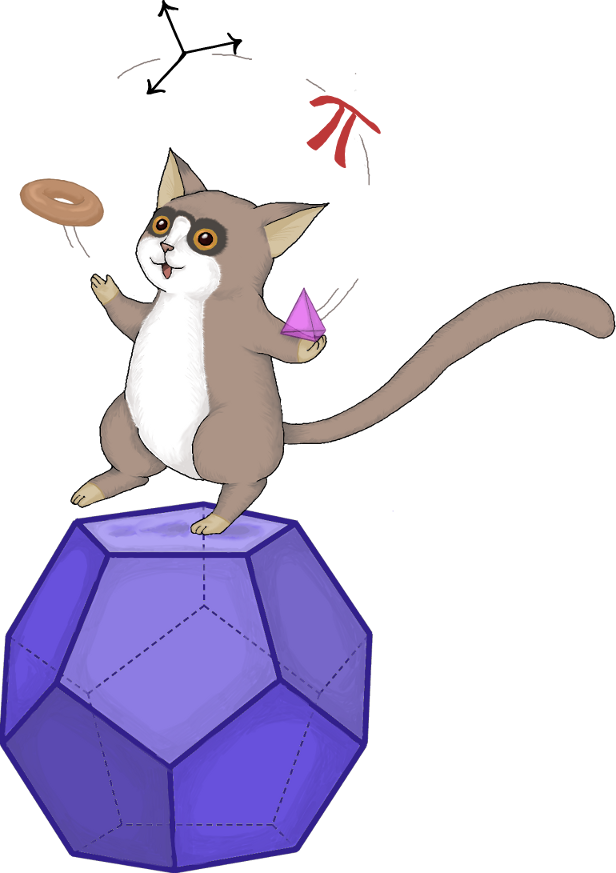
\includegraphics[scale=0.15]{gregor}
\end{center}

\begin{shaded}
  \begin{nota}
    Wir verwenden die folgenden Bezeichnungen:

    \begin{tabular}{ r l l }
      $\N$ & Menge der natürlichen Zahlen & $\{ 1, 2, 3, 4, ... \}$ \\
      $\Z$ & Menge der ganzen Zahlen & $\{ ..., -2, -1, 0, 1, 2, ... \}$ \\
      $\Q$ & Menge der rationalen Zahlen & $\tfrac{1}{3}, \tfrac{-17}{2}, 1 \in \Q$
    \end{tabular}
  \end{nota}
\end{shaded}


\datum{22. November 2013}

\section{Unmöglichkeitsbeweise über Invarianten}

\begin{wrapfigure}{r}{0.28\textwidth}
  \vspace{-24pt}
  \begin{center}
    \scalebox{0.8}{
      \newgame
      \showallbut{p,P,q,Q,b,B,k,K,r,R,n,N}
      \showboard
    }
  \end{center}
  \vspace{-50pt}
\end{wrapfigure}

Vor uns befindet sich ein leeres Schachbrett und ein großer Haufen Dominosteine. Ein Dominostein ist genauso groß wie zwei Felder des Schachbretts. Wenn du magst, kannst du dir das Schachbrett, die Dominosteine und ein paar Tetris-Steine (die übrigens auch Tetrominos genannt werden), die wir später noch brauchen werden, auf der Zirkel-Webseite\footnote{\mbox{\url{http://timbaumann.info/mathezirkel-kurs/invarianten-spiele.html}}} ausdrucken, ausschneiden und selbst mitknobeln.

\begin{frage}
  Ist es möglich, das Schachbrett mit Dominosteinen so zu belegen, dass jedes Feld bedeckts ist, keine zwei Dominosteine übereinander liegen und kein Stein über den Rand hinausragt? 
\end{frage}

\begin{antw}
  Ja. Lege in jede Zeile des Feldes 4 Dominosteine horizontal nebeneinander.
\end{antw}

Wir sägen nun aus dem Schachbrett die rechte untere Ecke, das Feld \emph{h1}, heraus.

\begin{frage}
  Ist es immer noch möglich, das Schachbrett wie beschrieben mit Dominosteinen zu belegen?
\end{frage}

\begin{antw}
  Nein. Das Schachbrett ohne rechte untere Ecke hat 63 Felder. Jeder Dominostein belegt genau zwei Felder. Wenn eine Überdeckung möglich wäre, so hätte das Schachbrett ohne rechte untere Ecke somit eine gerade Anzahl von Feldern. Also kann es keine Überdeckung geben.
\end{antw}

Während wir die erste Frage einfach positiv (bejahend) beantworten konnten, indem wir eine Überdeckung mit Dominosteinen angegeben haben, fällt uns die negative (verneinende) Antwort schwieriger: Wir mussten nämlich einen Grund finden, warum es eine solche Überdeckung nicht geben kann. Es reicht nicht aus, zu sagen, man habe keine Lösung gefunden. Es könnte ja immer noch sein, dass man sich nur ungeschickt angestellt hat und deshalb keine Lösung gefunden hat.

Wir sägen nun aus dem Schachbrett auch die linke obere Ecke, das Feld \emph{h8}, heraus.

\begin{frage}
  Wie immer: Gibt es nun eine Überdeckung des Schachbretts mit Dominosteinen?
\end{frage}

Das Schachbrett ohne die beiden Ecken hat wieder eine gerade Anzahl von Feldern, nämlich 62. Prinzipiell könnte also eine Überdeckung möglich sein. Aber wenn du versuchst, eine zu finden, wirst du feststellen dass, egal wie du dich anstellst, zwei Felder übrig bleiben. Du vermutest daher, dass es keine Lösung geben kann.

\begin{antw}
  Nein. Wenn man einen Dominostein auf das Brett legt, so bedeckt er, egal wie er liegt, ein weißes und ein schwarzes Feld. Die beiden Felder, die wir abgesegt haben, waren beides weiße Felder. Damit ist das um zwei Ecken verkleinerte Brett noch 30 weiße und 32 schwarze Felder. Jedes Mal, wenn wir einen Stein setzen, nimmt die Zahl der noch offenen weißen und die Zahl der noch offenen schwarzen Felder um je 1 ab. Nach drei gelegten Dominosteinen haben wir beispielsweise noch $30-3=27$ offene weiße und $32-3=29$ offene schwarze Felder. Zu jedem Zeitpunkt gibt es genau zwei schwarze unbedeckte Felder mehr als weiße unbedeckte Felder. Wenn alle weißen Felder bedeckt sind, gibt es also noch zwei schwarze offene Felder. Diese können aber nicht nebeneinander liegen, deshalb können sie nicht mit einem Domino überdeckt werden.
\end{antw}

Wären nicht zwei diagonal gegenüberliegende, sondern zwei Ecken, die an einer Seite liegen, herausgesägt worden, so wäre die Aufgabe lösbar gewesen. Bevor wir die Antwort etwas tiefer analysieren, wollen wir uns noch eine weitere Aufgabe anschauen:

\begin{aufg}
  Auf einer Insel leben 345 gelbe, 346 grüne und 347 blaue Chamäleons. Wann immer sich zwei Chamäleons gleicher Farbe begegnen, passiert nichts. Wenn sich aber zwei Chamäleons unterschiedlicher Farbe begegnen, so nehmen beide die dritte Farbe an. Beispielsweise hätten wir nach einem Treffen eines gelben und einer grünen Chamäleons nur noch 344 gelbe, 345 grüne, aber dafür 349 blaue Chamäleons. Frage: Ist es möglich, dass zu einem Zeitpunkt genau gleich viele Chamäleons jeder Farbe auf der Insel leben?
\end{aufg}

% Bildquelle: http://commons.wikimedia.org/wiki/File:Cham%C3%A4leon1.jpg
\begin{center}
  \raisebox{-0.4\height}{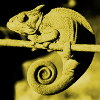
\includegraphics{chamaeleongelb}} + \raisebox{-0.4\height}{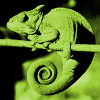
\includegraphics{chamaeleongruen}} $\longrightarrow$ $2 \cdot$ \raisebox{-0.4\height}{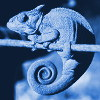
\includegraphics{chamaeleonblau}}
  \qquad
  \raisebox{-0.4\height}{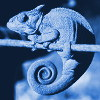
\includegraphics{chamaeleonblau}} + \raisebox{-0.4\height}{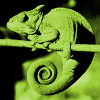
\includegraphics{chamaeleongruen}} $\longrightarrow$ $2 \cdot$ \raisebox{-0.4\height}{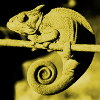
\includegraphics{chamaeleongelb}}
  \qquad
  \raisebox{-0.4\height}{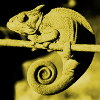
\includegraphics{chamaeleongelb}} + \raisebox{-0.4\height}{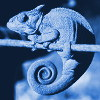
\includegraphics{chamaeleonblau}} $\longrightarrow$ $2 \cdot$ \raisebox{-0.4\height}{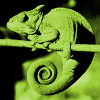
\includegraphics{chamaeleongruen}}
\end{center}

Grundsätzlich könnte diese Situation eintreten, da $345 + 346 + 347 = 1038$ durch $3$ teilbar ist. Wenn wir allerdings versuchen, eine Liste von Begegnungen zu erstellen, sodass nach diesen Begegnungen die Anzahl der Chamäleons jeder Farbe gleich ist, scheitern wir. Spoiler: Auch diese Aufgabe ist nicht lösbar.

Was haben diese Aufgaben gemeinsam? Zunächst haben wir eine Anfangssituation, beispielsweise das leere (verkleinerte) Schachbrett oder die Anzahlen der Fische jeder Farbe im Aquarium. Dann verändert sich die Ausgangslage durch Züge (das Legen eines Dominosteins) oder Ereignisse (Treffen von zwei Fischen). Die Frage in beiden Aufgaben ist, ob eine bestimmte Situation (alle Felder bedeckt bzw. gleich viele Fische von jeder Farbe) eintreten kann.

In beiden Aufgaben finden wir experimentell keine Lösung und suchen daher nach einem Grund, warum wir jedes solche Unterfangen von vornherein zum Scheitern verurteilt ist. In der Schachbrettaufgabe könnten wir dies begründen, indem wir alle Möglichkeiten ausprobieren. Davon gibt es allerdings ziemlich viele, sodass wir eine Antwort auf diesem Weg nur, wenn überhaupt, mit Hilfe eines Computers finden können. In der zweiten Aufgabe allerdings, gibt es (auf den ersten Blick) unendlich viele Möglichkeiten, wie sich Fische treffen können; wenn wir beispielsweise herausgefunden haben, dass wir mit 40 Treffen von Fischen die gewünschte Endsituation nicht erreichen können, so könnte uns das 41 Treffen zum Ziel führen.

Wir haben uns daher in der Aufgabe mit dem Schachbrett eines anderen Tricks bedient: Wir haben bemerkt, dass am Anfang das verkleinerte Brett $32 - 30 = 2$ schwarze Felder mehr besitzt als weiße Felder. Jedes Mal, wenn wir einen Dominostein gelegt haben, wurde ein weißes und ein schwarzes Feld verdeckt, also blieb die Differenz zwischen der Anzahlen der schwarzen offenen und weißen offenen Felder immer gleich. Wir haben also eine Zahl entdeckt, die wir für jedes unbedeckte, teilweise oder vollständig mit Steinen bedeckte Spielbrett ausrechnen können und die mit jedem weiteren platzierten Stein, egal wo er gelegt wird, gleich bleibt. Man sagt auch, dass diese Zahl unverändert (mit Fremdwort invariant) bleibt und nennt sie eine \emph{Invariante}. In der gewünschten Endposition, dass das ganze Brett belegt ist, wäre die Differenz zwischen den offenen schwarzen und offenen weißen Feldern gleich $0 - 0 = 0$. Diese Situation kann also beginnend bei unserer Anfangsposition nicht erreicht werden.

\begin{antw}
  Es ist nicht möglich, dass es irgendwann gleich viele Chamäleons von jeder Farbe gibt. Wir betrachten die Zahl $C$, die wir als Differenz zwischen der Anzahl der blauen und grünen Chamäleons festlegen. Zu Beginn ist $C = 347 - 346 = 1$. Wenn sich ein blaues und ein grünes Chamäleon treffen, so bleibt diese Zahl gleich. Wenn sich allerdings ein grünes und ein gelbes Chamäleon treffen, so nimmt die Zahl der grünen Chamäleons um eins ab, während die Zahl der blauen um zwei steigt. Insgesamt erhöht sich $C$ um drei. Wenn sich ein blaues und ein gelbes Chamäleon treffen, so sinkt $C$ um drei (mit ähnlicher Begründung). Die Zahl $C$ ist also nicht invariant. Aber wir stellen fest: Zu Beginn ist $C$ gleich 1, also nicht durch 3 teilbar. Wir wissen aber: Wenn eine ganze Zahl $k \in \Z$ durch 3 teilbar ist, so sind auch die Zahlen $k + 3$ und $k - 3$ durch 3 teilbar. Umgekehrt ist, wenn $k \in \Z$ nicht durch 3 teilbar ist, auch die Zahlen $k + 3$ und $k - 3$ nicht durch 3 teilbar. Also können wir folgern, dass nach jedem Treffen von zwei Chamäleons unsere Zahl immer noch \emph{nicht} durch 3 teilbar ist. Unsere Invariante ist hier also nicht die Zahl $C$ selbst, sondern die Tatsache, dass $C$ nicht durch 3 teilbar ist. In der gewünschten Endsituation wäre $C = 0$, da wir verlangen, dass die Zahl der blauen und grünen Chamäleons dann gleich ist. Aber 0 ist durch 3 teilbar! Folglich kann diese Situation nicht erreicht werden.
\end{antw}

Invarianten sind ein nützliches Mittel für Aufgaben obiger Art, bei denen man zeigen soll, dass eine bestimmte Situation nicht erreicht werden kann. Ein Nachteil dieser Technik ist es, dass Invarianten oft nicht offensichtlich sind, sondern es einiger Kreativität und Erfahrung bedarf, um sie zu finden. Bei der Schachbrettaufgabe könnte man feststellen, dass am Ende jedes Versuches zwei schwarze Felder übrig bleiben. Generell bietet sich an, wenn man so eine Aufgabe angeht, erst einmal rumzuprobieren und dabei Zahlen, die einem wichtig erscheinen, nach jedem Schritt aufzuschreiben und danach nach Mustern zu suchen.

Auch in der höheren Mathematik spielen Invarianten eine wichtige Rolle: Es gibt beispielsweise eine Teilgebiet der Mathematik, das sich mit Knoten befasst. Einen Knoten stellt man sich dabei als Seil im dreidimensionalen Raum vor, wobei Anfang und Ende des Seils zusammengebunden sind. Wenn wir einen Knoten haben, so stellen sich Mathematiker die Frage, ob wir diesen Knoten nur durch Bewegen des Seiles (ohne Zerschneiden) diesen Knoten auflösen können, sodass er nur noch aus einer einfachen Seilschlinge besteht. Um zu beweisen, dass dies für manche Knoten nicht möglich ist, haben Mathematiker Invarianten gefunden, die etwas komplizierter als unsere bisher gesehene Invarianten sind und beim Umformen eines Knoten gleich bleiben.

\begin{center}
  \scalebox{0.75}{
    \begin{tikzpicture}
      % L
      \fill [color=yellow,opacity=0.8] (0,0) -- ++ (2,0) -- ++ (0,1) -- ++ (-1,0) -- ++ (0,2) -- ++ (-1,0) -- cycle;
      \draw (0,0) -- ++ (2,0) -- ++ (0,1) -- ++ (-1,0) -- ++ (0,2) -- ++ (-1,0) -- cycle;
      \draw (0,0) ++ (0,2) -- ++ (1,0);
      \draw (0,0) ++ (0,1) -- ++ (1,0) -- ++ (0,-1);

      % Quadrat
      \fill [color=red,opacity=0.5] (3,0) -- (5,0) -- (5,2) -- (3,2) -- cycle;
      \draw (3,0) -- (5,0) -- (5,2) -- (3,2) -- cycle;
      \draw (3,0) ++ (1,0) -- ++ (0,2);
      \draw (3,0) ++ (0,1) -- ++ (2,0);

      % T
      \fill [color=blue,opacity=0.7] (7,0) -- ++ (1,0) -- ++ (0,3) -- ++ (-1,0) -- ++ (0,-1) -- ++ (-1,0) -- ++ (0,-1) -- ++ (1,0) -- cycle;
      \draw (7,0) -- ++ (1,0) -- ++ (0,3) -- ++ (-1,0) -- ++ (0,-1) -- ++ (-1,0) -- ++ (0,-1) -- ++ (1,0) -- cycle;
      \draw (7,0) ++ (1,1) -- ++ (-1,0) -- ++ (0,1) -- ++ (1,0);

      % I
      \fill [color=orange,opacity=0.7] (9,0) -- ++ (1,0) -- ++ (0,4) -- ++ (-1,0) -- cycle;
      \draw (9,0) -- ++ (1,0) -- ++ (0,4) -- ++ (-1,0) -- cycle;
      \draw (9,0) ++ (0,1) -- ++ (1,0);
      \draw (9,0) ++ (0,2) -- ++ (1,0);
      \draw (9,0) ++ (0,3) -- ++ (1,0);

      % Z
      \fill [color=green,opacity=0.7] (11,0) -- ++ (1,0) -- ++ (0,1) -- ++ (1,0) -- ++ (0,2) -- ++ (-1,0) -- ++ (0,-1) -- ++ (-1,0) -- cycle;
      \draw (11,0) -- ++ (1,0) -- ++ (0,1) -- ++ (1,0) -- ++ (0,2) -- ++ (-1,0) -- ++ (0,-1) -- ++ (-1,0) -- cycle;
      \draw (11,0) ++ (0,1) -- ++ (1,0) -- ++ (0,1) -- ++ (1,0);
    \end{tikzpicture}
  }
\end{center}

Oben siehst du die fünf verschiedenen Formen, die beim Spiel Tetris auftreten.

\begin{frage}
  Ist es möglich, aus den obigen fünf Figuren ein Rechteck zu legen? Dabei dürfen sich die Figuren nicht überlappen, aber beliebig oft gedreht oder gespiegelt werden.
\end{frage}

Zunächst einmal stellen wir fest, dass die fünf Figuren insgesamt $5 \cdot 4 = 20$ Felder belegen. Also muss das Rechteck, falls es existiert, entweder $1$ Feld breit und $20$ Felder lang oder $2$ Felder breit und $10$ Felder lang oder $4$ Felder breit und $5$ Felder lang sein. Offensichtlich scheidet die erste Möglichkeit aus. Man kann sich auch recht schnell überlegen, dass auch die zweite Möglichkeit nicht in Frage kommt (Tipp: platziere das orange Teil zuerst). Somit bleibt nur das $5 \times 4$-Rechtecks als Möglichkeit übrig. Wenn wir aber versuchen, solch ein Rechteck mit obigen Figuren zu belegen, scheitern wir immer wieder. Das hat auch einen Grund:

\begin{antw}
  Es ist nicht möglich, aus den Tetris-Figuren ein Rechteck zu legen. Wir legen die Figuren auf ein Schachbrett:

  \begin{center}
    \scalebox{0.75}{
      \begin{tikzpicture}
        \foreach \y in {-1,1,3}{
          \foreach \x in {-1,1,3,5,7,9,11}{
            \fill [color=black,opacity=0.8] (\x,\y) -- ++ (1,0) -- ++ (0,1) -- ++ (-1,0) -- cycle;
            \fill [color=black,opacity=0.8] (\x,\y) ++ (1,1) -- ++ (1,0) -- ++ (0,1) -- ++ (-1,0) -- cycle;
          }
          \fill [color=black,opacity=0.8] (13,\y) -- ++ (1,0) -- ++ (0,1) -- ++ (-1,0) -- cycle;
        }

        % L
        \fill [color=yellow,opacity=0.8] (0,0) -- ++ (2,0) -- ++ (0,1) -- ++ (-1,0) -- ++ (0,2) -- ++ (-1,0) -- cycle;
        \draw (0,0) -- ++ (2,0) -- ++ (0,1) -- ++ (-1,0) -- ++ (0,2) -- ++ (-1,0) -- cycle;
        \draw (0,0) ++ (0,2) -- ++ (1,0);
        \draw (0,0) ++ (0,1) -- ++ (1,0) -- ++ (0,-1);

        % Quadrat
        \fill [color=red,opacity=0.5] (3,0) -- (5,0) -- (5,2) -- (3,2) -- cycle;
        \draw (3,0) -- (5,0) -- (5,2) -- (3,2) -- cycle;
        \draw (3,0) ++ (1,0) -- ++ (0,2);
        \draw (3,0) ++ (0,1) -- ++ (2,0);

        % T
        \fill [color=blue,opacity=0.7] (7,0) -- ++ (1,0) -- ++ (0,3) -- ++ (-1,0) -- ++ (0,-1) -- ++ (-1,0) -- ++ (0,-1) -- ++ (1,0) -- cycle;
        \draw (7,0) -- ++ (1,0) -- ++ (0,3) -- ++ (-1,0) -- ++ (0,-1) -- ++ (-1,0) -- ++ (0,-1) -- ++ (1,0) -- cycle;
        \draw (7,0) ++ (1,1) -- ++ (-1,0) -- ++ (0,1) -- ++ (1,0);

        % I
        \fill [color=orange,opacity=0.7] (9,0) -- ++ (1,0) -- ++ (0,4) -- ++ (-1,0) -- cycle;
        \draw (9,0) -- ++ (1,0) -- ++ (0,4) -- ++ (-1,0) -- cycle;
        \draw (9,0) ++ (0,1) -- ++ (1,0);
        \draw (9,0) ++ (0,2) -- ++ (1,0);
        \draw (9,0) ++ (0,3) -- ++ (1,0);

        % Z
        \fill [color=green,opacity=0.7] (11,0) -- ++ (1,0) -- ++ (0,1) -- ++ (1,0) -- ++ (0,2) -- ++ (-1,0) -- ++ (0,-1) -- ++ (-1,0) -- cycle;
        \draw (11,0) -- ++ (1,0) -- ++ (0,1) -- ++ (1,0) -- ++ (0,2) -- ++ (-1,0) -- ++ (0,-1) -- ++ (-1,0) -- cycle;
        \draw (11,0) ++ (0,1) -- ++ (1,0) -- ++ (0,1) -- ++ (1,0);

        \fill [color=white,path fading=fade right] (-1.1,-1) rectangle ++ (1,6);
        \fill [color=white,path fading=fade left] (13.1,-1) rectangle ++ (1,6);
        \fill [color=white,path fading=fade top] (-1,-1.1) rectangle ++ (15,1);
        \fill [color=white,path fading=fade bottom] (-1,4.1) rectangle ++ (15,1);
      \end{tikzpicture}
    }
  \end{center}
  Nun fällt etwas auf: Alle Figuren bis auf die blaue belegen je zwei weiße und zwei schwarze Felder (egal, wie man sie hinlegt). Die blaue Figur, jedoch, belegt drei weiße Felder und nur ein schwarzes Feld (oder umgekehrt). Damit belegen die Figuren zusammengenommen ungleich viele weiße wie schwarze Felder, egal wie man sie anordnet. Damit kann man insbesondere kein $4 \times 5$-Rechteck mit ihnen legen, denn jedes $4 \times 5$-Rechteck auf einem Schachfeld hat gleich viele weiße und schwarze Felder.
\end{antw}

\datum{6. und 20. Dezember 2013, 10. Januar 2014}

\section{Rechnen mit Restklassen}

\subsection{Teilbarkeit}

\begin{defn}
  Eine Zahl $b \in \Z$ ist durch $a \in \Z$ \emph{teilbar}, wenn es eine Zahl $c \in Z$ gibt mit
  \[ a \cdot c = b. \]
\end{defn}

\begin{nota}
  Wir verwenden dann die Kurzschreibweise $a \divides b$, gesprochen "`$a$ teilt $b$"'. Wir sagen auch, dass $a$ ein \emph{Teiler} von $b$ ist oder dass $b$ ein Vielfaches von $a$ ist. Im Fall, dass die Zahl $a$ die Zahl $b$ \emph{nicht} teilt, d.\,h. keine Zahl $c \in \Z$ existiert mit $a \cdot c = b$, schreiben wir $a \not\divides b$.
\end{nota}

\begin{bsp}
  Folgende Aussagen stimmen:
  \begin{multicols}{5}
    \begin{itemize}
      \item $3 \divides 6$
      \item $5 \not\divides 13$
      \item $8 \divides -8$
      \item $3 \divides 12345$
      \item $2 \not\divides 1001$
    \end{itemize}
  \end{multicols}
\end{bsp}

\begin{exkurs}
  Der Ausdruck $a \divides b$ ist eine mathematische Aussage. Andere Beispiele für mathematische Aussagen sind:
  \begin{itemize}
    \begin{multicols}{4}
      \item $\sqrt{2}$ ist irrational
      \item $3 > 5$
      \item $n$ ist gerade
      \item $m$ ist eine Primzahl
    \end{multicols}
    \item Jeder Winkel lässt sich mit Zirkel und Lineal halbieren.
    \item Für $n \in \N$ mit $n \geq 2$ gibt keine Zahlen $a, b, c \in \N$, sodass $a^n + b^n = c^n$ stimmt.
    \item Es gibt unendlich viele Primzahlenzwillinge, das sind Primzahlen $p$ und $q$, mit $q = p + 2$.
  \end{itemize}

  Mathematische Aussagen können richtig oder falsch sein. Beispielsweise ist in den obigen Beispielen die erste wahr, die zweite falsch und über die nächsten beiden können wir nichts sagen, da sie Zahlen $n$ und $m$ beinhalten, die erst noch genauer definiert werden müssen. Die vorletzte Aussage trägt den Namen "`Fermats letzter Satz"' und ist richtig, doch hat es über 300 Jahre gedauert, bis sie bewiesen werden konnte. Von der letzten Aussage wird vermutet, dass sie stimmt, es existiert jedoch kein Beweis.
\end{exkurs}

\begin{frage}
  Gibt es eine Zahl $a \in \Z$, die Teiler von $0$ ist, d.\,h. $a \divides 0$?
\end{frage}

\begin{antw}
  Ja, wir können sogar jede beliebige Zahl $a \in Z$ nehmen: Setze $c \coloneqq 0$, dann ist $a \cdot c = a \cdot 0 = 0$ und somit ist die Definition erfüllt.
\end{antw}

\begin{frage}
  Gibt es andersherum eine Zahl $b \in \Z$, die durch $0$ teilbar ist, also $0 \divides b$?
\end{frage}

\begin{antw}
  Ja, aber nur die Zahl $0$ selber. Mit $a = 0$, ist für ein beliebiges $c$ nämlich $a \cdot c = 0 \cdot c = 0$, also muss $b = 0$ sein.
\end{antw}

\begin{exkurs}
  Sei $z \in \Z$ eine ganze Zahl. Wenn $z$ ungerade ist, so ist $z$ nicht durch $8$ teilbar. Um nicht immer "`wenn ..., dann ..."' schreiben zu müssen, verwenden Mathematiker folgende Notation:

  \[ z \text{ ist ungerade } \implies 8 \not\divides z \]

  Dabei stehen auf der linken und rechten Seite des $\Rightarrow$-Zeichens mathematische Aussagen $P$ und $Q$. Die Zeile $(P \Rightarrow Q)$ ist wiederum selbst eine mathematische Aussage, nämlich die Aussage, dass wenn $P$ stimmt, dann auch $Q$ stimmt. Dabei ist es wichtig, dass links $P$ steht und rechts $Q$, denn in unserem Beispiel stimmt die Aussage andersrum nicht: Wenn $z$ nicht durch $8$ teilbar ist, dann muss $z$ noch nicht unbedingt ungerade sein. Zum Beispiel ist $z = 4$ nicht durch $8$ teilbar, aber gerade.

  Ein anderes Beispiel: Eine ganze Zahl $m$ ist ungerade, wenn die Zahl $(m{+}1)$ gerade ist. Andersrum ist $(m{+}1)$ gerade, wenn $m$ ungerade ist. Hier ist also die Umkehrung erfüllt, im Gegensatz zum vorherigen Beispiel. Also ist $m$ immer dann und nur dann ungerade, wenn $(m{+}1)$ ungerade ist. Mathematiker verwenden dafür eine besondere Notation:
  \[ n \text{ ist ungerade } \quad \iff \quad (n + 1) \text{ ist gerade } \]
  Auf beiden Seiten des $\Leftrightarrow$-Zeichens stehen dabei wieder mathematische Aussagen. Der Pfeil $\Leftrightarrow$ bedeutet, dass die linke Aussage nur dann stimmt, wenn die rechte Aussage stimmt.
\end{exkurs}

Wir wollen nun ein paar Tatsachen über die Teilbarkeit beweisen.

\begin{satz}
  Seien $n, p, q \in \Z$ ganze Zahlen. Dann gilt:
  \begin{satzliste}
    \item $n \divides p \text{ und } p \divides q \implies n \divides q$
    \item $n \divides p \implies n \divides (p \cdot q)$
    \item $n \divides p \text{ und } n \divides q \implies n \divides (p + q)$
  \end{satzliste}
\end{satz}

\begin{proof}
  \begin{beweisliste}
    \item Aus der Definition von Teilbarkeit wissen wir, dass es $c, d \in \Z$ gibt mit
    \[ n \cdot c = p \quad \text{und} \quad p \cdot d = q \]
    Um zu zeigen, dass $n \divides q$ gilt, müssen wir nach derselben Definition eine Zahl für die Leerstelle finden, sodass die Gleichung
    \[ n \cdot \leer = q \]
    erfüllt ist. Wir behaupten, dass die Zahl $p \coloneqq (c \cdot d)$ dies leistet. Wir rechnen nämlich nach:
    \[ n \cdot (c \cdot d) = \underbrace{(n \cdot c)}_{= p} \cdot d = p \cdot d = q. \]
    Dabei haben wir im ersten Schritt das Assoziativgesetz gebraucht.
    \item Aus der Definition von Teilbarkeit erhalten wir ein $c \in \Z$ mit
    \[ n \cdot c = p. \]
    Wir müssen folgene Leerstelle sinnvoll ersetzen:
    \[ n \cdot \leer = p \cdot q. \]
    Wir nehmen dafür die Zahl $(c \cdot q)$ und rechnen
    \[ n \cdot (c \cdot q) = \underbrace{(n \cdot c)}_{= p} \cdot q = p \cdot q \]
    \item Aus der Definition erhalten wir $c, d \in \Z$ mit
    \[ n \cdot c = p \quad \text{und} \quad n \cdot d = q. \]
    Es soll folgende Gleichung gelten:
    \[ n \cdot \leer = p + q \]
    Wir setzen $(c+d)$ für $\leer$ und rechnen
    \[ n \cdot (c+d) = \underbrace{n \cdot c}_{= p} + \underbrace{n \cdot d}_{= q} = p + q. \]
    Im ersten Schritt haben wir dabei das Distributivgesetz angewendet.
  \end{beweisliste}
\end{proof}

\begin{acht}
  Folgendes Rechengesetz gilt \emph{nicht}:
  \[ p \divides n \text{ und } q \divides n \implies (p \cdot q) \divides n \]
  Ein Gegenbeispiel dafür ist $p = 4, q = 6, n = 12$.
\end{acht}

\begin{exkurs}
  In den natürlichen Zahlen $\N$, den ganzen Zahlen $\Z$ und den rationalen Zahlen $\Q$ gelten folgende Rechenregeln:
  \begin{itemize}
    \item \emph{Kommutativgesetz}: $a + b = b + a$ und $a \cdot b = b \cdot a$
    \item \emph{Assoziativgesetz}: $a + (b + c) = (a + b) + c$ und $a \cdot (b \cdot c) = (a \cdot b) \cdot c$
    \item \emph{Distributivgesetz}: $a \cdot (b + c) = a \cdot b + a \cdot c$
  \end{itemize}
  Es ist eine gute Übung, sich zu überlegen, welche Plus- und Mal-Zeichen wir durch Minus- und Divisions-Zeichen ersetzen dürfen, sodass die Regeln immer noch stimmen.
\end{exkurs}

\subsection{Restklassen}

Übungszettel vom 10. Januar 2014: \mbox{\url{http://timbaumann.info/mathezirkel-kurs/uebung4.pdf}}

Sei $n$ eine natürliche Zahl und $p, q$ natürliche Zahlen, die bei der Division durch $n$ den gleichen Rest $r$ haben, also
\begin{align*}
  p : n &= a \text{ Rest } r \\
  q : n &= b \text{ Rest } r
\end{align*}
für zwei Zahlen $a, b \in \Z$. Wir können dabei außerdem annehmen, dass $r$ eine Zahl zwischen $0$ bis $n - 1$ ist (warum?). Wenn wir obige Gleichungen umschreiben, erhalten wir
\begin{align*}
  p &= n \cdot a + r, \\
  q &= n \cdot b + r.
\end{align*}
Wir rechnen:
\[ p - q = (n \cdot a + r) - (n \cdot b + r) = n \cdot a + r - n \cdot b - r = n \cdot a + n \cdot b = n \cdot (a + b). \]
Wir haben also $n \cdot (a+b) = p - q$, folglich nach Definition von Teilbarkeit $n \divides (p - q)$. Dies ist unser erstes halbwegs interessantes Ergebnis: Zwei Zahlen $p$ und $q$, die bei Division durch $n$ den gleichen Rest haben, unterscheiden sich nur durch ein Vielfaches von $n$.

\begin{defn}
  Für zwei Zahlen $p$ und $q$, die sich nur durch ein Vielfaches von $n \in N$ unterscheiden (d.\,h. $n \divides (p-q)$) schreiben wir
  \[ p \equiv q \pmod{n}. \]
  Wir sprechen: "`$p$ ist gleich $q$ modulo $n$"'.
\end{defn}

\begin{nota}
  Falls $p \equiv q \pmod{n}$ nicht stimmt, schreiben wir $p \not\equiv q \pmod{n}$.
\end{nota}

\begin{bsp}
  Folgende Aussagen stimmen:
  \begin{itemize}
    \begin{multicols}{3}
      \item $1 \equiv 4 \pmod{3}$
      \item $0 \equiv 16 \pmod{8}$
      \item $-4 \equiv 3 \pmod{7}$
      \item $-1001 \equiv -1003 \pmod{2}$
      \item $4 \not\equiv 2 \pmod{4}$
      \item $0 \not\equiv -101 \pmod{3}$
    \end{multicols}
  \end{itemize}
\end{bsp}

\begin{acht}
  Wir dürfen den Teil in Klammern auf keinen Fall weglassen! Es gilt nämlich
  $4 \equiv 7 \pmod{3}$, aber nicht $4 \equiv 7 \pmod{6}$!
\end{acht}

\begin{satz}
  Sei $n \in \N$ und $a, a_1, a_2, b, b_1, b_2, c \in \Z$ ganze Zahlen. Dann gilt:
  \begin{satzliste}
    \item $a \equiv a \pmod{n}$
    \item $a \equiv b \pmod{n} \text{ und } b \equiv c \pmod{n} \implies a \equiv c \pmod{n}$
    \item $a_1 \equiv a_2 \pmod{n} \text{ und } b_1 \equiv b_2 \pmod{n} \implies a_1 + b_1 \equiv a_2 + b_2 \pmod{n}$
    \item $a_1 \equiv a_2 \pmod{n} \text{ und } b_1 \equiv b_2 \pmod{n} \implies a_1 \cdot b_1 \equiv a_2 \cdot b_2 \pmod{n}$
  \end{satzliste}
\end{satz}

\begin{proof}
  \begin{beweisliste}
    \item Es ist $a - a = 0$ und somit gilt $n \divides (a - a)$, da $0$ von jeder beliebigen Zahl geteilt wird.
    \item Es gilt nach Voraussetzung $n \divides (a-b)$ und $n \divides (b-c)$, also nach unserem Wissen über Teilbarkeit
    \[ n \divides \underbrace{\left((a-b) + (b-c)\right)}_{= (a - c)}. \]
    \item Nach Voraussetzung gilt $n \divides (a_1 - a_2)$ und $n \divides (b_1 - b_2)$. Somit
    \[ n \divides \underbrace{\left((a_1 - a_2) - (b_1 - b_2)\right)}_{= (a_1 + b_1) - (a_2 + b_2)}. \]
    \item Nach Voraussetzung gilt $n \divides (a_1 - a_2)$ und $n \divides (b_1 - b_2)$. Somit gilt auch
    \[ n \divides (a_1 - a_2) \cdot b_1 \quad \text{und} \quad n \divides a_2 \cdot (b_1 - b_2), \]
    also auch $n \divides ((a_1 - a_2) \cdot b_1 + a_2 \cdot (b_1 - b_2))$. Es gilt aber
    \[ (a_1 - a_2) \cdot b_1 + a_2 \cdot (b_1 - b_2) = a_1 \cdot b_1 - a_2 \cdot b_1 + a_2 \cdot b_1 - a_2 \cdot b_2 = a_1 \cdot b_1 - a_2 \cdot b_2, \]
    somit ist dies gleichbedeutend zu $n \divides (a_1 \cdot b_1 - a_2 \cdot b_2)$.\qedhere
  \end{beweisliste}
\end{proof}

\begin{defn}
  Sei $n \in \N$ eine natürliche und $a \in \Z$ eine ganze Zahl.
  Die \emph{Restklasse} von $a$ modulo $n$ ist nun die Menge aller Zahlen, die gleich $a$ modulo $n$ sind, also
  \[ \overline{a} \coloneqq \{ z \in Z \mid z \equiv a \!\!\!\pmod{n} \}. \]
\end{defn}

\begin{shaded}
  \begin{nota}
    Obige Notation bedeutet: Die Menge aller Zahlen $z \in \Z$, die die Bedingung rechts neben dem Mittelstrich erfüllen, also $z \equiv a \pmod{n}$.
  \end{nota}
\end{shaded}

\begin{aufg}
  Überzeuge dich davon, dass gilt:
  \[ \overline{a} = \{ ..., a + (-3) \cdot n, a + (-2) \cdot n, a + (-1) \cdot n, a, a + 1 \cdot n, a + 2 \cdot n, a + 3 \cdot n, ... \}. \]
  Folgere, dass es genau $n$ verschiedene Restklassen modulo $n$ gibt und dass jede ganze Zahl in genau einer Restklasse enthalten ist.
\end{aufg}

\begin{bsp}
  Auf dem Zahlenstrahl unten sind alle Zahlen in einer Restklasse modulo $3$ in der gleichen Farbe hinterlegt:
  \begin{center}
    \begin{tikzpicture}
      \foreach \i in {-7,-4,-1,2,5}{
        \fill [color=blue,opacity=0.4] (\i,0) circle (12pt);
        \fill [color=orange,opacity=0.4] (\i+1,0) circle (12pt);
        \fill [color=yellow,opacity=0.4] (\i+2,0) circle (12pt);
      }
      \foreach \i in {-7,-6,...,7}{
        \node at (\i,0) {$\i$};
        \draw [thick] (\i,-0.5) ++ (0,-0.125) -- ++ (0,0.25);
      }
      \draw [thick,<->] (-8,-0.5) -- (8,-0.5);
    \end{tikzpicture}
  \begin{minipage}{0.3\linewidth}
    $\overline{0} = \{ ..., -6, -3, 0, 3, 6, ... \}$
  \end{minipage}
  \begin{minipage}{0.3\linewidth}
    $\overline{1} = \{ ..., -5, -2, 1, 4, 7, ... \}$
  \end{minipage}
  \begin{minipage}{0.3\linewidth}
    $\overline{2} = \{ ..., -7, -4, -1, 2, 5, ... \}$
  \end{minipage}
  \end{center}
\end{bsp}

\vspace{10pt}

% Uhrenanalogie?

Mit Restklassen können wir auch die Chamäleons-Aufgabe genauer analysieren: In der Lösung dieser Aufgabe haben wir $C$ als die Differenz zwischen der Anzahl der blauen und grünen Chamäleons festgelegt. Zu Beginn ist diese $C = 347 - 346 = 1$. Wir haben festgestellt, dass diese Zahl bei jeder Begegnung von Chamäleons gleichbleibt, um drei steigt oder um drei sinkt. Also verlässt diese Zahl die Restklasse der Zahl $1$ modulo $3$ nicht. Insbesondere wird $C$ niemals den Wert $0$ annehmen, da dieser nicht in der Restklasse der Zahl $1$ modulo $3$ enthalten ist.

\iffalse
\begin{defn}
  Für $n \in \N$ und $r \in \{ 0, 1, ..., n-1 \}$
\end{defn}

\begin{bsp}
  Du kennst Restklassen aus dem Alltag: $4$ Uhr nachmittags und $16$ Uhr sind Bezeichnungen für diesselbe Uhrzeit, da
  \[ 16 \equiv 4 \pmod{12}. \]
\end{bsp}
\fi

\begin{satz}
  Für alle $n \in \N$ gilt
  \[ 10^n \equiv 1\underbrace{00\cdots0}_{n \text{ Nullen}} \equiv 1 \pmod{3} \]
\end{satz}

\begin{proof}
  Es gilt
  \[ \underbrace{99 \cdots 9}_{n \text{ Neuner}} = 3 \cdot \underbrace{33 \cdots 3}_{n \text{ Dreier}}, \]
  also $3 \divides 99 \cdots 9$ bzw. $99 \cdots 9 \equiv 0 \pmod{3}$. Wir rechnen:
  \[ 10^n \equiv \underbrace{99 \cdots 9}_{n \text{ Neuner}} + 1 \equiv 0 + 1 \equiv 1 \pmod{3}.\qedhere \]
\end{proof}

Du kennst wahrscheinlich folgenden Test auf Teilbarkeit durch $3$: Er besagt, dass eine Zahl genau dann durch $3$ teilbar ist, wenn ihre Quersumme durch $3$ teilbar ist. Vielleicht hast du dich auch schon einmal gefragt, warum dieser Test funktioniert. Mit der Vorarbeit, die wir bisher geleistet haben, fällt ein Beweis nicht schwer:

\begin{satz}
  Sei $a \in \Z$ eine ganze Zahl, wobei die Ziffern von $a$ im Zehnersystem $a_n, ..., a_0$ seien, also $a = a_n \cdot 10^n + a_{n-1} \cdot 10^{n-1} + ... + a_1 \cdot 10 + a_0$. Die Quersumme von $a$ ist dann gegeben durch $\mathrm{QS}(a) = a_n + a_{n-1} + ... + a_1 + a_0$. Es gilt dann
  \[ a \equiv \mathrm{QS}(a) \pmod{3}. \]
\end{satz}

\begin{proof}
  Es gilt für alle $i$ zwischen $0$ und $n$
  \[ a_i \cdot 10^i \equiv a_i \cdot 1 \equiv a_i \pmod{3} \]
  durch Anwenden der letzten Behauptung und den Modulo-Rechenregeln. Also haben wir
  \[ a \equiv a_n \cdot 10^n + ... + a_1 \cdot 10 + a_0 \equiv a_n + ... + a_1 + a_0 \equiv \mathrm{QS}(a) \pmod{3}. \qedhere \]
\end{proof}

Das ist nicht ganz die Behauptung des Quersummentests, allerdings ist $m \in \Z$ genau dann durch $3$ teilbar, wenn $m \equiv 0 \pmod{3}$. Falls aber $\mathrm{QS}(a)$ durch $3$ teilbar ist, so haben wir $\mathrm{QS}(a) \equiv 0$ und es folgt mit der ersten Modulo-Rechenregel schon
\[ a \equiv \mathrm{QS}(a) \equiv 0 \pmod{3}. \]

In beiden obigen Behauptungen kann man auch die Zahl $3$ durch die Zahl $9$ ersetzen, ohne dass dadurch die Behauptungen falsch werden (gehe die Beweise durch und überlege dir, warum das möglich ist). Somit erhalten wir einen Test auf Teilbarkeit durch $9$: Eine Zahl ist genau dann durch $9$ teilbar, wenn ihre Quersumme durch $9$ teilbar ist.

Es gibt auch einen ganz ähnlichen Test für Teilbarkeit durch $11$: Eine Zahl $a \in \Z$ ist genau dann durch $11$ teilbar, wenn die alternierende Quersumme durch $11$ teilbar ist. Sei $a = a_n \cdot 10^n + ... + a_1 \cdot 10 + a_0$, dann ist die alternierende Quersumme von $a$
\[ \mathrm{AQS}(a) = a_0 - a_1 + a_2 - a_3 + ... \pm a_n. \]
Wenn $n$ gerade ist, steht dabei ein Plus-Zeichen vor $a_n$, sonst ein Minuszeichen. Das Wort alternierend deutet an, dass wir abwechselnd die Ziffern, beginnend bei der letzten, dazuzählen und abziehen.

Zum Beispiel ist $\mathrm{AQS}(1234321) = 1 - 2 + 3 - 4 + 3 - 2 + 1 = 0$ und da $0$ durch $11$ teilbar ist, ist auch $1234321$ durch $11$ teilbar.

Wir wollen nun beweisen, dass dieser Teilbarkeitstest immer richtig funktioniert. Dazu zunächst eine Vorüberlegung:

\begin{satz}
  Für alle $n \in \N$ gilt
  \[
    10^n \equiv 1\underbrace{00\cdots0}_{n \text{ Nullen}} \equiv \begin{cases}
      10 \equiv -1, & \text{falls $n$ ungerade}\\
      1, & \text{falls $n$ gerade}
    \end{cases} \pmod{11}
  \]
\end{satz}

\begin{proof}
  Zunächst einmal gilt, wie man leicht nachrechnet, $100 \equiv 1 \pmod{11}$ und $10 \equiv -1 \pmod{11}$. Die Behauptung stimmt also schon mal für $n{=}1$ und $n{=}2$. Für beliebige gerade $n$ folgt nun:
  \[ 10^n \equiv 100^{\frac{n}{2}} \equiv \underbrace{100 \cdot 100 \cdot ... \cdot 100}_{\text{$\tfrac{n}{2}$ Hunderter}} \equiv 1 \cdot 1 \cdot ... \cdot 1 \equiv 1 \pmod{11}. \]
  Für ungerade Zahlen $n$ rechnen wir analog:
  \[ 10^n \equiv 10 \cdot 100^{\frac{n-1}{2}} \equiv 10 \cdot \underbrace{100 \cdot 100 \cdot ... \cdot 100}_{\text{$\tfrac{n-1}{2}$ Hunderter}} \equiv 10 \cdot 1 \cdot 1 \cdot ... \cdot 1 \equiv 10 \equiv -1 \pmod{11}.\qedhere \]
\end{proof}

\begin{satz}
  Sei $a \in \Z$ eine ganze Zahl, wobei die Ziffern von $a$ im Zehnersystem $a_n, ..., a_0$ seien, also $a = a_n \cdot 10^n + a_{n-1} \cdot 10^{n-1} + ... + a_1 \cdot 10 + a_0$. Dann gilt:
  \[ a \equiv \mathrm{AQS}(a) \pmod{11}. \]
\end{satz}

\begin{proof}
  Es gilt für alle $i$ zwischen $0$ und $n$
  \[ a_i \cdot 10^i \equiv \begin{cases} a_i \cdot (-1) \equiv -a_i, & \text{falls $i$ ungerade} \\ a_i \cdot 1 \equiv a_i, & \text{falls $i$ gerade} \end{cases} \pmod{3} \]
  durch Anwenden der letzten Behauptung und den Modulo-Rechenregeln. Also haben wir
  \[ a \equiv a_0 + a_1 \cdot 10 + ... + a_n \cdot 10^n \equiv a_0 - a_1 + ... \mp a_{n-1} \pm a_n \equiv \mathrm{AQS}(a) \pmod{11}, \]
  wobei $a_n$ addiert wird, falls $n$ gerade ist, sonst subtrahiert.
\end{proof}

Inbesondere folgt: Die Zahl $a$ ist genau dann durch $11$ teilbar (also $a \equiv 0 \pmod{11}$), wenn $AQS(a)$ durch $11$ teilbar ist (also $AQS(a) \equiv 0 \pmod{11}$).

\datum{24. Januar 2014}

\section{Nim-Spiele}

Folgendes Spiel könnte dir bekannt vorkommen:

Auf einem Haufen liegt eine Anzahl von Steinen. Zwei Spieler sind abwechselnd an der Reihe und dürfen in jedem Zug einen, zwei oder drei Steine vom Haufen nehmen. Verloren hat derjenige Spieler, für den keine Steine mehr übrig sind (also hat der Spieler gewonnen, der den letzten Stein vom Haufen nimmt).

Betrachten wir folgende Spielsituation: Auf dem Haufen liegen noch genau vier Steine und dein Gegner ist an der Reihe. Er kann in diesem Zug nicht gewinnen, da er maximal drei Steine vom Haufen nehmen darfst. Nach seinem Zug allerdings werden nur noch ein, zwei oder drei Steine auf dem Haufen sein, je nachdem, ob er in diesem Zug drei, zwei oder einen Stein nimmt. Diese restlichen Steine kannst du in deinem nächsten Zug nehmen und hast gewonnen.

Also solltest du versuchen, dafür zu sorgen, dass nach einem deiner Züge genau vier Steine auf dem Haufen liegen. Dann hast du automatisch gewonnen. Wie können wir dieses Ziel erreichen? Dafür betrachten wir eine weitere Spielsituation:

Auf dem Steinhaufen liegen genau acht Steine. Dein Gegner ist an der Reihe. Nach seinem Zug liegen entweder fünf, sechs oder sieben Steine auf dem Haufen. Du kannst dann einen, zwei bzw. drei Steine nehmen, sodass nach deinem Zug noch genau vier Steine auf dem Haufen liegen. Damit hast du gewonnen.

Wenn nun auf dem Haufen zwölf Steine liegen und dein Gegner an der Reihe ist, dann kannst du dafür sorgen, dass nach seinem und deinem Zug acht Steine auf dem Haufen sind.

Allgemeiner hast du eine Strategie zu gewinnen, wenn dein Gegner an der Reihe ist und die Anzahl der Steine ein Vielfaches von vier ist, bzw. du an der Reihe bist und die Anzahl an Steinen kein Vielfaches von vier ist. Du musst dabei einfach, wenn du an der Reihe bist, so viele Steine nehmen, sodass die Anzahl auf dem Haufen ein Vielfaches von vier ist.

\begin{aufg}
  Spiele dieses Spiel gegen deine Freunde/Eltern/Geschwister und beobachte, wie lang sie brauchen, bis sie die Strategie verstanden haben.
\end{aufg}

Wir wollen nun ein ähnliches Spiel analysieren:

Auf dem Tisch liegen mehrere Steinhaufen. Wir zuvor sind die beiden Spieler abwechselnd an der Reihe. Sie suchen sich in jedem Zug einen Steinhaufen aus. Dann dürfen sie von diesem (und nur von diesem Haufen) eine beliebige Anzahl von Steinen nehmen. Dabei müssen sie mindestens einen und können maximal alle Steine dieses Haufens nehmen. Wie im vorherigen Spiel hat derjenige Spieler verloren, der keinen Zug mehr machen kann.

Für dieses Spiel gibt es ebenfalls eine Gewinnstrategie. Diese benötigt sogenannte Binärzahlen:

\begin{exkurs}
  Wenn wir Zahlen schreiben, verwenden wir normalerweise die üblichen zehn Ziffern. Der Trick, mit dem man auf einheitliche und elegante Weise mit diesen zehn Ziffern auch Zahlen schreiben kann, die viel größer sind als $neun$, stammt aus Indien: Eine Ziffer repräsentiert eine unterschiedliche Anzahl, je nachdem, wo sie in der Zahl steht. Die Ziffer ganz rechts repräsentiert Einer, die Ziffer weiter links davon Zehner, die nächste Ziffer Hunderter und so weiter. Allgemeiner gilt für eine $n$-stellige Zahl $a$ mit Ziffern $a_0, ..., a_n \in \{ 0, 1, 2, ..., 9 \}$, wobei $a_0$ die Ziffer ganz rechts sei:
  \[ a = a_n \cdot 10^n + a_{n-1} \cdot 10^{n-1} + ... + a_1 \cdot 10 + a_0. \]
  Aber warum gerade zehn Ziffern? Nun, das hat keinen besonderen Grund abgesehen davon, das dies eine Zahl ist, die gewissermaßen auf der Hand liegt: Der Mensch hat nunmal zehn Finger und zehn Zehen (nicht umsonst bedeutet das englische Wort ``digit'' sowohl Finger als auch Ziffer). Wir können genauso gut ein Zahlensystem entwickeln, das mit nur zwei Ziffern auskommt, sagen wir den Ziffern $0$ und $1$. Die Zahlen null bis zwölf in diesem System sind:
  \[ 0, 1, 10, 11, 100, 101, 110, 111, 1000, 1001, 1010, 1011, 1100 \]
  Für die Zahlen null und eins konnten wir direkt die Ziffern verwenden. Für die Zahl zwei benötigen wir bereits die "`Zweierstelle"' und ab der Zahl vier die "`Viererstelle"'. Dieses System, das nur mit $0$ und $1$ auskommt, wird \emph{Binärsystem} genannt. Im Gegensatz dazu heißt das übliche System mit $10$ Ziffern \emph{Dezimalsystem}. In diesem System gilt für eine $n$-stellige Zahl $a$ mit Ziffern $a_0, ..., a_n \in \{ 0, 1 \}$:
  \[ a = a_n \cdot 2^n + a_{n-1} \cdot 2^{n-1} ... + a_1 \cdot 2 + a_0. \]
\end{exkurs}

\begin{aufg}
  Rechne um!
  \begin{itemize}
    \item Vom Dezimal- ins Binärsystem:
      \begin{inparaenum}[\itshape a\upshape)]
        \item $13$
        \item $-5$
        \item $21$
        \item $64$
      \end{inparaenum}
    \item Vom Binär- ins Dezimalsystem:
      \begin{inparaenum}[\itshape a\upshape)]
        \item $11111$
        \item $1101$
        \item $-11010$
        \item $10101010$
      \end{inparaenum}
  \end{itemize}
\end{aufg}

Nun wollen wir das Spiel mit Hilfe von Binärzahlen analysieren: Angenommen, du bist dran und auf dem Tisch liegen drei Haufen von Steinen. Wir schreiben neben jeden Haufen die Anzahl von Steinen als Zahl im Binärsystem:

\begin{center}
  \begin{tabular}{ >{$}r<{$} | l }
    \text{Anzahl} & Haufen\\
    \hline
    110 & \steinhaufen{6}\\
    11 & \steinhaufen{3}\\
    1010 & \steinhaufen{10}
  \end{tabular}
\end{center}

Achte darauf, dass dabei alle Binärzahlen rechts ausgerichtet sind und die Einerstelle, die Zweierstelle, die Viererstelle usw. der Binärzahlen in einer Spalte untereinander stehen. Nun betrachten wir jede Spalte für sich genommen und zählen in dieser Spalte die Anzahl der Einsen. Was für uns wichtig ist, ist ob diese Anzahl gerade oder ungerade ist. Oben haben wir vier Spalten (da die größte Zahl von Steinen in einem Haufen, die Zehn, vier Binärziffern lang ist): in der ersten steht nur eine Eins, ebenso in der zweiten und vierten Spalte. In der dritten Spalte stehen drei Einsen. Also steht in jeder Spalte eine ungerade Anzahl von Einsen. Unser Ziel ist es, zu erreichen, dass in jeder Spalte eine gerade Anzahl an Einsen steht. Warum wir das wollen wird gleich klarwerden. Wie können wir dieses Ziel erreichen? Wir könnten im obigen Beispiel die $1010$ durch eine eine $101$ ersetzen. Da $101$ im Binärsystem für die Fünf steht, müssten wir somit vom Haufen mit zehn Steinen fünf Steine wegnehmen, sodass fünf Steine übrig bleiben.

Gibt es immer solch einen Zug, der dafür sorgt, dass in jeder Spalte eine gerade Anzahl von Einsen steht? Ja, immer dann, wenn dies vor unserem Zug nicht der Fall ist. Ermittele dazu die erste Spalte von links, in der eine ungerade Anzahl an Einsen steht, und wähle einen Haufen aus, dessen Zeile in dieser Spalte eine Eins stehen hat (warum gibt es einen solchen immer?). Im Beispiel oben ist das der letzte Haufen mit zehn Steinen, da dies die einzige Zeile in der Tabelle ist, in der die Binärzahl vier Ziffern lang ist. Wir können die Ziffern dieser Binärzahl so verändern, sodass danach in jeder Spalte eine gerade Anzahl an Einsen steht. Dabei wird die Zahl auch immer kleiner, denn die erste Ziffer (von links) die wir verändern, ist eine Eins. Sie wird zu einer Null. Egal, wie sich die Ziffern rechts davon ändern, die Zahl wird dadurch kleiner als die ursprüngliche Zahl. Eine ähnliche Situation ist die folgende: Wenn sich zwei Dezimalzahlen nur in der Einerstelle, Zehnerstelle und Hunderterstelle voneinander unterscheiden, aber die erste Zahl auf der Hunderterterstelle eine Vier und die zweite Zahl dort eine Drei stehen hat, dann ist die erste Zahl auf jeden Fall größer als die zweite. Um dies zu entscheiden mussten wir uns gar nicht erst die Zehner- und die Einerstelle ansehen.

Bleibt noch zu erklären, warum wir überhaupt erreichen wollen, dass die Anzahl von Einsen nach unserem Zug in jeder Spalte gerade ist. Dazu überlegen wir, was nach dem Zug unseres Gegners der Fall sein wird: Der Gegner muss von genau einem Haufen Steine entfernen. Dadurch ändert er in der Binärdarstellung der Anzahl der Steine dieses Haufens mindestens eine Ziffer. Dadurch wird die Anzahl der Einsen in mindestens einer Spalte wieder ungerade. Dann können wir mit unserem Zug wieder erreichen, dass die Anzahl an Einsen in jeder Spalte gerade ist. Der darauffolgende Zug des Gegners wird wieder dafür sorgen, dass die Anzahl an Einsen in mindestens einer Spalte ungerade ist, usw. Also ist jedes Mal, wenn wir an der Reihe sind, die Anzahl an Einsen in mindestens einer Spalte ungerade. Aber dann können nicht alle Haufen leer sein! Das heißt, wir können mit dieser Strategie nicht verlieren. Also gewinnen wir damit.

Wenn beide Spieler diese Strategie kennen, dann hängt der Ausgang des Spiels nur von der Anfangssituation ab: Wenn zu Beginn die Anzahl von Einsen in jeder Spalte gerade ist, dann verliert der Spieler, der anfängt, sonst gewinnt er.

\begin{aufg}
  Wer gewinnt in den folgenden Spielsituationen, wenn du und dein Gegner die Gewinnstrategie kennen und du an der Reihe bist?

  \adjustbox{valign=t}{\begin{minipage}{0.28\linewidth}
    \begin{tabular}{ >{$}r<{$} | l }
      \text{Anzahl} & Haufen\\
      \hline
      1 & \steinhaufen{1}\\
      10 & \steinhaufen{2}\\
      11 & \steinhaufen{3}\\
      100 & \steinhaufen{4}\\
      101 & \steinhaufen{5}
    \end{tabular}
  \end{minipage}}
  \adjustbox{valign=t}{\begin{minipage}[t]{0.4\linewidth}
    \begin{tabular}{ >{$}r<{$} | l }
      \text{Anzahl} & Haufen\\
      \hline
      1001 & \steinhaufen{9}\\
      11 & \steinhaufen{3}\\
      1 & \steinhaufen{1}\\
      1011 & \steinhaufen{11}
    \end{tabular}
  \end{minipage}}
  \adjustbox{valign=t}{\begin{minipage}[t]{0.4\linewidth}
    \begin{tabular}{ >{$}r<{$} | l }
      \text{Anzahl} & Haufen\\
      \hline
      1001 & \steinhaufen{9}\\
      1001 & \steinhaufen{9}\\
      111 & \steinhaufen{7}\\
      111 & \steinhaufen{7}\\
    \end{tabular}
  \end{minipage}}

  \vspace{8pt}

  Zusatzfrage: Gibt es in der letzten Spielsituation auch noch eine einfachere Spielstrategie für deinen Gegenspieler?
\end{aufg}

\begin{aufg}
  Spiele dieses Spiel gegen deine Freunde/Eltern/Geschwister. Erkläre ihnen nach einigen Runden die Gewinnstrategie.
\end{aufg}

\datum{7. und 21. Februar 2014}

\section{Vollständige Induktion}

Übungszettel vom 7. Februar 2014: \mbox{\url{http://timbaumann.info/mathezirkel-kurs/uebung5.pdf}}

Vollständige Induktion ist eines der grundlegenden mathematischen Beweisverfahren. Vollständige Induktion benutzt man immer dafür, um zu zeigen, dass eine bestimmte Aussage für alle natürlichen Zahlen gilt. Zum Beispiel:

\begin{aufg}
  Zeige, dass für alle natürlichen Zahlen $n \in \N$ die folgende Formel gilt:

  \[ \frac{1}{2^1} + \frac{1}{2^2} + \frac{1}{2^3} + ... + \frac{1}{2^{n-1}} + \frac{1}{2^n} = 1 - \frac{1}{2^n}. \]
\end{aufg}

Wir können nun hergehen und diese Formel für spezielle Werte von $n$ nachrechnen, z.\,B. für $n=1$ oder $n=5$ oder (mithilfe eines Computers) für alle natürlichen Zahlen $n$ kleiner als eine Million.

Wir können uns auch intuitiv klar machen, warum diese Formel gilt: Wir stellen uns einen Zahlenstrahl vor. Wir beginnen bei der Zahl $\frac{1}{2}$. Dann addieren wir $\frac{1}{4}$, also die Hälfte des Abstands von $\frac{1}{2}$ zu $1$. Wir befinden uns dann bei $\frac{3}{4}$. Dann addieren wir $\frac{1}{8}$, also die Hälfte des Abstandes von $\frac{3}{4}$ zu $1$. Wenn wir so weitermachen, halbiert sich der Abstand von unserer aktuellen Zahl zur Zahl $1$ in jedem Schritt. Und das ist ziemlich genau die Aussage der Aufgabe.

Nun ist aber das Nachrechnen der Formel für konkrete natürliche Zahlen kein Beweis der Aufgabe. Wir können schließlich nicht die Formel für alle natürlichen Zahlen durch einzelnes Nachrechnen prüfen, denn es gibt ja unendlich viele natürliche Zahlen. Die zweite Überlegung ist schon deutlich näher an einem mathematischen Beweis (der nachfolgende Beweis folgt in gewisser Weise sogar den gleichen Überlegungen). Wir wollen nun die Aufgabe mathematisch ganz korrekt durch vollständige Induktion beweisen. Um uns das Leben einfacher zu machen, führen wir davor aber noch etwas Notation ein:

\begin{shaded}
  \begin{nota}
    In obiger Aufgabe summieren wir
    \[ \frac{1}{2^1} + \frac{1}{2^2} + \frac{1}{2^3} + ... + \frac{1}{2^{n-1}} + \frac{1}{2^n} = 1 - 2^n, \]
    also alle Brüche $\frac{1}{2^k}$, wobei $k$ nacheinander die Werte $1$ bis $n$ annimmt. Für solche Summen verwendet man folgende abkürzende Schreibweise:
    \[ \sum_{k=1}^n \frac{1}{2^k} = \frac{1}{2^1} + \frac{1}{2^2} + \frac{1}{2^3} + ... + \frac{1}{2^{n-1}} + \frac{1}{2^n} = 1 - 2^n. \]

    Der griechische Buchstabe $\Sigma$ heißt Sigma, die Zeilen $k=1$ darunter und $n$ darüber bedeuten, dass zuerst $k=1$, dann $k=2$, usw. bis $k=n$ gilt. Die Variable $k$ wird auch Zählvariable genannt. Die Werte des Ausdrucks $\frac{1}{2^k}$ rechts neben $\Sigma$ werden für all diese Werte von $k$ aufaddiert.

    Mit dieser Notation wird die Formel einfacher und damit überschaubarer. Außerdem spart man sich viele Auslassungspunkte.

    Weitere Beispiele für die Verwendung dieser Summennotation sind:

    \begin{align*}
      \sum_{k=1}^5 k &= 1 + 2 + 3 + 4 + 5 = 15 \\
      \sum_{k=0}^n 2^i &= 2^0 + 2^1 + 2^2 + ... + 2^n \\
      \sum_{j=1}^k \frac{1}{j} &= \frac{1}{1} + \frac{1}{2} + \frac{1}{3} + ... + \frac{1}{k}
    \end{align*}

    Das letzte Beispiel zeigt, das wir für die Zählvariable auch andere Buchstaben außer $k$ benutzen können, und statt bis $n$ auch bis $k$ summieren können.
  \end{nota}
\end{shaded}

Wir können damit die obige Aufgabe folgendermaßen umschreiben:

\begin{aufg}
  Zeige, dass für alle natürlichen Zahlen $n \in \N$ die folgende Formel gilt:
  \[ \sum_{k=1}^n \frac{1}{2^k} = 1 - 2^n. \]
\end{aufg}

\begin{proof}
  Wir führen Induktion über $n$ durch:

  \emph{Induktionsanfang:} Die Formel stimmt für $n=1$, wie wir leicht nachrechnen:
  \[ \sum_{k=1}^n \frac{1}{2^k} = \sum_{k=1}^1 \frac{1}{2^k} = \frac{1}{2^1} = 1 - \frac{1}{2^1} = 1 - \frac{1}{2^n} \]

  \emph{Induktionsschritt:} Wir nehmen an, dass die Formel für eine bestimmte natürliche Zahl $n \in \N$ gilt und zeigen, dass die Formel dann auch für die nächstgrößere natürliche Zahl, also $n{+}1$, gilt. Dazu rechnen wir:
  \[ \sum_{k=1}^{n+1} \frac{1}{2^k} = \left( \sum_{k=1}^{n} \frac{1}{2^k} \right) + \frac{1}{2^{n+1}} = \left( 1 - \frac{1}{2^n} \right) + \frac{1}{2^{n+1}} = 1 - \frac{2}{2^{n+1}} + \frac{1}{2^{n+1}} = 1 - \frac{1}{2^{n+1}} \]
  Bei der ersten Gleichheit steht dabei auf beiden Seiten genau dasselbe, nur jeweils mit etwas anderer Notation. Links wurde die Summennotation für das Addieren von $n+1$ Zahlen verwendet, rechts nur für $n$ Zahlen. Dafür wurde rechts der letzte Summand extra hinzuaddiert. Die zweite Gleichheit folgt aus der Annahme (s.\,o.), dass die Formel aus der Aufgabe für die Zahl $n$ stimmt. Wir konnten also die Formel direkt für den eingeklammerten Ausdruck anwenden. Die restlichen Gleichheiten sind Routine-Rechnungen.
\end{proof}

Warum nun ist dies ein korrekter Beweis für die Aufgabe? Nun, wir können dem Beweis direkt entnehmen, dass die Formel für die kleinste natürliche Zahl, also $n=1$ gilt. Das haben wir im Teil "`Induktionsanfang"' direkt nachgerechnet. Dann gilt aber auch die Formel für $n=2$, denn: Die Formel gilt für $n=1$ und das Argument im Teil "`Induktionsschritt"' sagt uns, dass deswegen auch die Formel für $1+1=2$ gilt. Dann gilt aber auch die Formel für $n=3$, denn: Die Formel gilt für $n=2$ und das Argument im Teil "`Induktionsschritt"' sagt uns, dass deswegen auch die Formel für $2+1=3$ gilt. Dann gilt aber auch die Formel für $n=4$, denn: Die Formel gilt für $n=3$ und das Argument im Teil "`Induktionsschritt"' sagt uns, dass deswegen auch die Formel für $3+1=4$ gilt. Und so weiter und so fort. Da wir so jede natürliche Zahl erreichen können, gilt die Formel für alle natürliche Zahlen.

Wir wollen nochmal allgemein zusammenfassen, wie ein Beweis durch vollständige Induktion aufgebaut ist. Wenn wir eine mathematische Aussage für alle natürlichen Zahlen $n \in \N$ beweisen wollen, dann reicht es aus, zu zeigen:

\begin{itemize}
  \item Die Aussage gilt für die kleinste natürliche Zahl $n$, also $n=1$ (\emph{Induktionsanfang})
  \item Wenn die Aussage für eine natürliche Zahl $n$ gilt, dann gilt sie auch für die nächstgrößere natürliche Zahl $n+1$ (\emph{Induktionsschritt}).
\end{itemize}

Im Induktionsschritt dürfen wir also voraussetzen, dass die Aussage, die wir zeigen wollen, für die Zahl $n$ gilt. Diese Voraussetzung nennt man auch \emph{Induktionsannahme} oder \emph{Induktionshypothese}. Unsere Aufgabe ist es, zu zeigen, dass die Aussage dann auch für $n+1$ gilt.

\begin{exkurs}
  Vollständige Induktion wird oft schlicht auch nur Induktion genannt. Das Adjektiv "`vollständig"' dient zur Abgrenzung der mathematischen Induktion von der philosophischen Induktion, einem Prinzip des Schlussfolgerns, dass die Ableitung von abstrakten Gesetzmäßigkeiten von konkreten Beobachtungen beschreibt.
\end{exkurs}

Am besten versteht man Induktion und wann man sie wirkungsvoll einsetzt, indem man Aufgaben rechnet. Darum:

\begin{aufg}
  Zeige: Für alle natürlichen Zahlen $n \in \N$ gilt:
  \[ \sum\limits_{k=1}^n k = \frac{n \cdot (n+1)}{2}. \]
\end{aufg}

Zu dieser Aufgabe gibt es eine Geschichte, die in vielen Mathematik-Büchern zu finden ist: Der später berühmte Mathematiker Carl Friedrich Gauß bekam als Schüler von seinem Lehrer die Aufgabe, alle Zahlen von $1$ bis $100$ zu addieren. Der Lehrer hatte damit gerechnet, dass seine Klasse mit dieser Aufgabe einige Zeit beschäftigt sein würde. Umso verblüffter war er, als der kleine Gauß schon nach kurzer Zeit die Lösung hatte: $\sum_{i=1}^{100} i = 5050$. Wie hatte Gauß diese Aufgabe so schnell gelöst? Seine Idee war, die Zahlen von $1$ bis $101$ in folgende Paare aufzuteilen:

\[
  \begin{matrix}
    1 & 2 & 3 & \cdots & 49 & 50 \\
    + & + & + & \cdots & + & + \\
    100 & 99 & 98 & \cdots & 52 & 51 \\
    = & = & = & \cdots & = & = \\
    101 & 101 & 101 & \cdots & 101 & 101
  \end{matrix}
\]

Die Summe jedes Paares ist dabei $101$. Wir man leicht sieht, gibt es genau $50$ solcher Paare. Also ist die Summe aller Zahlen von $1$ bis $100$ gleich $50 \cdot 101 = 5050$.

Wir können auch in die Formel aus der Aufgabe $n = 100$ setzen und kommen so auf diesselbe Lösung. Der Term $\frac{n \cdot (n+1)}{2}$ lässt sich (für gerade Zahlen $n$) folgendermaßen interpretieren: Es gibt $\frac{n}{2}$ Paare von Zahlen, deren Summe jeweils $n+1$ ist.

Die Begründung der Formel mittels Zahlenpaare wir oben funktioniert für gerade Zahlen. Man kann sich auch überlegen, dass die Formel auch für ungerade Zahlen gilt. Diese Überlegungen bilden zusammen schon einen Beweis der Formel. Einen alternativen Beweis kann man per Induktion führen:

\begin{proof}
  \emph{Induktionsanfang:} Die Formel stimmt für $n=1$, denn
  \[ \sum\limits_{k=1}^n k = \sum\limits_{k=1}^1 = 1 = \frac{1 \cdot 2}{2} = \frac{n \cdot (n+1)}{2}. \]
  \emph{Induktionsschritt:} Angenommen, die Formel gilt für die natürliche Zahl $n$, also $\sum_{k=1}^n k = \frac{n \cdot (n+1)}{2}$. Wir müssen zeigen, dass die Formel dann auch für $n+1$ stimmt, also dass gilt:
  \[ \sum\limits_{k=1}^{n+1} k = \frac{(n+1) \cdot ((n+1)+1)}{2} \quad \left(= \frac{(n+1) \cdot (n+2)}{2} \right). \]
  Dies können wir mithilfe der Induktionshypothese leicht nachrechnen:
  \begin{align*}
    \sum\limits_{k=1}^{n+1} k &= \sum\limits_{k=1}^{n} k + (n+1) \overset{\text{IH}}{=} \frac{n \cdot (n+1)}{2} + (n+1) = \frac{n \cdot (n+1)}{2} + \frac{2 \cdot (n+1)}{2} =\\
    &= \frac{n \cdot (n+1) + 2 \cdot (n+1)}{2} = \frac{(n+2) \cdot (n+1)}{2} = \frac{(n+1) \cdot (n+2)}{2}.
  \end{align*}
  Bei der ersten Gleichheit steht auf beiden Seiten wieder genau dasselbe, nur mit anderer Notation. Bei der mit IH beschrifteten Gleichheit habe wir die Induktionshypothese (abgekürzt IH) gebraucht. Hinter der vorletzten Gleichheit steckt das Distributiv-, hinter der letzten Gleichheit das Kommutativgesetz.
\end{proof}

Bislang haben wir mit Induktion nur Aufgaben gelöst, in denen man eine Gleichheit zeigen sollte. Man Induktion aber auch für Ungleichungen anwenden:

\begin{aufg}
  Zeige: Für alle natürlichen Zahlen $n \geq 4$ gilt:
  \[ n! \geq 2^n \geq n^2. \]
\end{aufg}

\begin{shaded}
  \begin{erinn}
    Der Ausdruck $n!$ (für eine natürliche Zahl $n$) wird "`$n$ Fakultät"' ausgesprochen und ist definiert als das Produkt aller Zahlen von $1$ bis $n$, also
    \[ n! \coloneqq 1 \cdot 2 \cdot ... \cdot n. \]
    Man setzt üblicherweise $0! \coloneqq 0$. Es gilt dann offensichtlich für alle $n \geq 1$: $n! = n \cdot (n-1)!$

    Die Fakultät wird häufig für die Beantwortung von Aufgaben wie "`Wie viele Möglichkeiten gibt es, $n$ Personen auf $n$ Sitzplätze zu verteilen"' gebraucht (Antwort: $n!$).

    Außerdem: Der Doppelpunkt vor dem Gleichheitszeichen weißt darauf hin, dass die Gleichheit nicht aufgrund einer Rechnung, sondern nach Definition gilt. Wir legen also den Ausdruck links des $\coloneqq$-Zeichens durch den Ausdruck rechts davon fest.
  \end{erinn}
\end{shaded}

Abgesehen davon, dass wir es in dieser Aufgabe nicht mit einer Gleichheit zu tun haben, in der auf der linken Seite eine Summe vorkommt, hat diese Aufgabe noch einen anderen Unterschied zu den bisher gerechneten Aufgaben: Bis jetzt sollten wir zeigen, dass eine Formel für alle natürlichen Zahlen gilt. In dieser Aufgabe sollen wir die Ungleichung nicht für alle natürlichen Zahlen, sondern nur für alle natürlichen Zahlen, die größer oder gleich $4$ sind, zeigen. Für die Zahlen $1$, $2$ und $3$ ist die Behauptung nämlich schlicht falsch:

\begin{center}
  \begin{tabular}{| >{$}l<{$} | >{$}r<{$} | >{$}r<{$} | >{$}r<{$} |}
    \hline
    n & n! & 2^n & n^2\\
    \hline
    0 & 1 & 1 & 0\\
    1 & 1 & 2 & 1\\
    2 & 2 & 4 & 4\\
    3 & 6 & 8 & 9\\
    4 & 24 & 16 & 16\\
    5 & 120 & 32 & 25\\
    \hline
  \end{tabular}
\end{center}

In der Aufgaben müssen wir genau genommen zwei Ungleichungen zeigen: Die erste Ungleichung $n! \geq 2^n$ und die zweite Ungleichung $2^n \geq n^2$ für je $n \geq 4$.
Wir können beide Ungleichungen jeweils einzeln wie die vorherigen Aufgaben mit Induktion beweisen, mit dem Unterschied, dass wir die Induktion bei der Zahl $4$ starten:

\begin{proof}
  \begin{itemize}
    \item Erste Ungleichung $(n! \geq 2^n)$:

    \emph{Induktionsanfang} ($n=4$): Durch Rechnung:
    \[ n! = 4! = 4 \cdot 3 \cdot 2 \cdot 1 = 24 \geq 16 = 2^4 = 2^n. \]

    \emph{Induktionsschritt} ($n \to n{+}1$, wobei $n \geq 4$): Wir rechnen:
    \[ (n+1)! = (n+1) \cdot n! \overset{\text{IH}}{\geq} (n+1) \cdot 2^n \geq 2 \cdot 2^n = 2^{n+1}. \]
    In dieser Rechnung haben wir folgende Tatsache zweimal gebraucht: Für drei positive natürliche (oder auch rationale oder reelle Zahlen) $a, b, c$ gilt: Wenn $a \geq b$ ist, dann ist auch $a \cdot c \geq b \cdot c$. Hinter dieser der ersten Ungleichung steckt die Induktionshypothese, dass $n! \geq 2^n$, zusammen mit dieser Tatsache ($a = n!$, $b = 2^n$, $c = n+1$). Die zweite Annahme folgt mit $n+1 \geq n \geq 4 \geq 2$ und der Tatsache angewendet auf $a = n{+}1$, $b = 2$ und $c = n{+}1$.

    \item Um die zweite Ungleichung zu beweisen, brauchen wir noch eine weitere Ungleichung, die wir per Induktion beweisen, nämlich: Für alle $n \geq 3$ gilt $2^n \geq 2n + 1$ (Hilfsbehauptung).

    \emph{Induktionsanfang} ($n=3$): Durch Rechnung:
    \[ 2^n = 2^3 = 8 \geq 7 = 2 \cdot 3 + 1 = 2 \cdot n + 1. \]

    \emph{Induktionsschritt} ($n \to n{+}1$, wobei $n \geq 3$):
    \begin{align*}
      2^{n+1} = 2 \cdot 2^n &\overset{\text{IH}}{\geq} 2 \cdot (2n + 1) = 4n + 2 \geq 2n + 2 + n = 2 \cdot (n+1) + n \geq\\
      &\geq 2 \cdot (n+1) + 3 \geq 2 \cdot (n+1) + 1.
    \end{align*}

    \item Zweite Ungleichung $(2^n \geq n^2)$:

    \emph{Induktionsanfang} ($n=4$): Durch Rechnung:
    \[ 2^n = 2^4 = 16 = 4^2 = n^2. \]
    Da also $2^n = n^2$, gilt auch $2^n \geq n^2$ ($=$ ist ein Spezialfall von $\geq$).

    \emph{Induktionsschritt} ($n \to n{+}1$, wobei $n \geq 4$): Hier ist es einfacher, von hinten nach vorne zu rechnen, also $(n+1)^2 \leq 2^{n+1}$ zu zeigen:
    \[ (n+1)^2 = n^2 + 2n + 1 \overset{\text{IH}}{\leq} 2^n + 2n + 1 \leq 2^n + 2^n = 2 \cdot 2^n = 2^{n+1}. \]
    Die Gültigkeit des ersten $\leq$-Zeichens folgt aus unserer Induktionshypothese ($2^n \geq n^2$), die des zweiten $\leq$-Zeichens durch unsere Hilfsbehauptung, die wir gerade eben in Punkt zwei bewiesen haben.\qedhere
  \end{itemize}
\end{proof}

Folgende Aufgabe stammt (leicht abgewandelt) aus der 51. Mathematik-Olympiade. Obwohl sie eine Aufgabe für die 11. bis 13. Klasse ist, lässt sie sich sehr einfach durch Induktion lösen:

% 51. Mathematik-Olympiade, 2. Stufe (Regionalrunde), Klasse 11-13, Aufgabe 511324
\begin{aufg}[Turnier]
  In einem Fechtturnier mit $2^n$ Teilnehmern kämpft jeder Fechter genau einmal gegen jeden anderen. Kein Kampf endet unentschieden. Eine Reporterin möchte nacheinander Einzelinterviews mit $n+1$ Fechtern führen. Diese sollen so ausgewählt werden, dass jeder interviewte Fechter gegen alle Fechter, die vor ihm interviewt wurden, gesiegt hat.

  Zeige, dass für alle natürlichen Zahlen $n$ die Reporterin eine entsprechende Auswahl von Fechtern für die Interviews treffen kann.
\end{aufg}

\begin{proof}
  \emph{Induktionsanfang} ($n=1$): Dann gibt es $2^n = 2^1 = 2$ Fechter, die Reporterin will $n+1 = 1+1 = 2$ Fechter, also alle beide interviewen. Es findet genau ein Fechtkampf statt. Die Reporterin erreicht ihr Ziel, wenn sie zuerst den Verlierer, dann den Gewinner interviewt.

  \emph{Induktionsschritt} ($n \to n{+}1$): Es kämpfen insgesamt $2^{n+1}$ Fechter gegeneinander, also jeder Fechter gegen die anderen $2^{n+1} - 1$ Fechter. Durchschnittlich gewinnt jeder Fechter die Hälfte seiner Duelle, also $\frac{2^{n+1} - 1}{2} = \frac{2^{n+1}}{2} - \frac{1}{2} = 2^n - \frac{1}{2}$ viele. Da dieser Durchschnitt keine ganze Zahl ist, muss es mindestens einen Fechter geben, der mindestens $2^n$ (die nächstgrößere ganze Zahl über $2^n - \frac{1}{2}$) Duelle gewonnen hat. Unter den $2^n$ Verlierern dieser Duelle kann die Reporterin nach Induktionsannahme eine gewünschte Reihenfolge von $n$ Interviewpartnern finden. Wenn sie danach den Sieger dieser Duelle, also den Fechter, der gegen die $2^n$ zuvor interviewten Fechter gewonnen hat, interviewt, hat sie ihr Ziel erreicht.
\end{proof}

\begin{wrapfigure}{r}{0.22\textwidth}
  \vspace{-15pt}
  \begin{center}
    \begin{tikzpicture}[shorten >=1pt,->]
      \tikzstyle{vertex}=[circle,fill=black!25,minimum size=17pt,inner sep=0pt]

      \foreach \name/\angle/\text in {P-1/234/1, P-2/162/2, 
                                      P-3/90/3, P-4/18/4, P-5/-54/5}
        \node[vertex,xshift=6cm,yshift=.5cm] (\name) at (\angle:1cm) {$\text$};

      \foreach \from/\to in {1/2,2/3,3/4,4/5,1/5,1/3,2/4,3/5,1/4,5/2}
        { \draw (P-\from) -- (P-\to); }
    \end{tikzpicture}
  \end{center}
  \vspace{-15pt}
\end{wrapfigure}

Auf der rechten Seiten siehst du einen gesättigten gerichteten Graphen mit 5 Knoten (graue Kreise). Die Pfeile zwischen den Knoten werden auch {\em Kanten} genannt. Wir sagen, dass wir einen Knoten $B$ von einem anderen Knoten $A$ direkt erreichen können, wenn eine Kanten von A nach B verläuft (also die Pfeilspitze zu B zeigt). Ein Knoten $B$ kann von einem anderen Knoten $A$ in zwei Schritten erreicht werden, wenn es einen Knoten $C$ gibt, sodass $C$ von $A$ direkt erreichbar ist und $B$ von $C$ direkt erreichbar ist.

Im Beispiel ist der Knoten $3$ vom Knoten $1$ in zwei Schritten erreichbar, aber andersrum der Knoten $1$ nicht vom Knoten $3$ in zwei Schritten erreichbar. Außerdem ist der Knoten $2$ von jedem anderen Knoten in höchstens zwei Schritten erreichbar.

\begin{aufg}
  Zeige, dass es in jedem gesättigten gerichteten Graphen mit $n$ Knoten einen Knoten gibt, der von jedem anderen Knoten in höchstens zwei Schritten erreicht werden kann.
\end{aufg}

\begin{proof}
  \emph{Induktionsanfang} ($n=1$): Wir haben also nur einen Knoten im Graph. Dieser kann offensichtlich von jedem anderen Knoten erreicht werden, denn es gibt ja gar keinen anderen Knoten.

  \emph{Induktionsschritt} ($n \to n{+}1$):
  Wir greifen uns aus einem gesättigten Graphen mit $n+1$ Knoten einen Knoten $K$ wahllos heraus. Die restlichen $n$ Knoten und deren Knoten untereinander bilden einen gerichteten Graphen mit $n$ Knoten. Nach Induktionsannahme gibt es unter ihnen einen Knoten, der von den restlichen $n-1$ Knoten in höchstens zwei Schritten erreicht werden kann. Wir nennen diesen Knoten $A$. Die Knoten, die direkt mit $A$ verbunden sind, nennen wir D-Knoten ("`D"' für direkt). Nun fügen wir den am Anfang herausgenommenen Knoten $K$ und all seine Kanten wieder hinzu. Es tritt nun einer der folgenden zwei Fälle ein:
  \begin{itemize}
    \item Alle D-Knoten und auch $A$ sind direkt mit $K$ verbunden. Dann ist $K$ ein Knoten, wie er in der Aufgabenstellung gesucht wird.
    \item Entweder ist $K$ direkt mit $A$ verbunden, oder es gibt einen D-Knoten, zu dem $K$ direkt verbunden ist (also existiert eine Kante von $K$ zu einem D-Knoten). In beiden Fällen ist der Knoten $A$ von $K$ in höchstens zwei Schritten erreichbar. Da $A$ auch von jedem anderen Knoten in höchstens $2$ Schritten erreichbar ist, ist $A$ der gesuchte Knoten.\qedhere
  \end{itemize}
\end{proof}

\begin{shaded}
  \begin{acht}
    Nicht alle Induktionsbeweise, die du in Büchern findest, folgen in allen Details dem hier vorgestellten Schema. Insbesondere wird im Induktionsschritt oft gezeigt, dass eine Aussage für die Zahl $n$ ($n \geq 2$) gilt, wenn die Aussage für die Zahl $n{-}1$ gilt. Man schließt im Induktionsschritt also nicht von $n$ auf $n{+}1$, sondern von $n{-}1$ auf $n$. Für die Gültigkeit der Induktion spielt das aber keine Rolle. Als Beispiel ist die nächste Aufgabe mit dieser Konvention bearbeitet.
  \end{acht}
\end{shaded}

\begin{wrapfigure}{r}{0.12\textwidth}
  \vspace{-30pt}
  \begin{center}
    \scalebox{0.75}{
      \begin{tikzpicture}
        \draw (0,0) -- ++ (2,0) -- ++ (0,1) -- ++ (-1,0) -- ++ (0,1) -- ++ (-1,0) -- cycle;
        \draw (0,0) ++ (1,0) -- ++ (0,1) -- ++ (-1,0);
        \fill [color=blue,opacity=0.6] (0,0) -- ++ (2,0) -- ++ (0,1) -- ++ (-1,0) -- ++ (0,1) -- ++ (-1,0) -- cycle;
      \end{tikzpicture}
    }
  \end{center}
  \vspace{-35pt}
\end{wrapfigure}

Ein Tromino ist ein Stein, der zwei Schachbrettfelder breit und zwei Schachbrettfelder hoch ist und genau drei Schachbrettfelder überdeckt, also gewissermaßen ein $(2 \times 2)$-Quadrat, aus dem eine Ecke entfernt wurde (siehe rechts). 

\begin{aufg}
  Zeige per Induktion, dass es für alle $n \in \N$ möglich ist, ein quadratisches Brett, das $2^n$ Felder breit und hoch ist, und aus dem eine Ecke entfernt wurde, mit Trominos zu belegen.
\end{aufg}

\begin{proof}
  \emph{Induktionsanfang} ($n=1$): Dann ist das Brett je $2^n = 2^1 = 2$ Felder lang und breit, wobei eine Ecke herausgeschnitten ist. Kurz: Das Feld hat die Form eines Trominos.

  \emph{Induktionsschritt} ($n{-}1 \to n$, wobei $n \geq 2$): Wir beschriften ein $(2^k \times 2^k)$-Brett, aus dem eine Ecke entfernt wurde, mit $F^k$. Nach Induktionsvoraussetzung ist also das Brett $F^{n-1}$ mit Trominos belegbar und wir müssen zeigen, dass auch das Brett $F^n$ mit Trominos belegt werden kann. Dazu teilen wir das Brett $F^n$ in vier quadratische Stücke mit Seitenlänge $2^{n-1}$. Dabei entsteht ein $F^{n-1}$-Brett und drei vollständige $(n{-}1 \times n{-}1)$-Bretter (mit allen Ecken). Wir legen ein Tetromino in die Mitte des $F^n$-Bretts, sodass es je eine Ecke der drei vollständigen $(n{-}1 \times n{-}1)$-Bretter bedeckt. Damit bleiben uns noch vier $F^{n-1}$-Bretter übrig, die wir nach Induktionsannahme belegen können.
\end{proof}

\begin{center}
  \scalebox{0.80}{
    \begin{tikzpicture}
      \draw (0,0) -- ++ (4,0) -- ++ (0,3.5) -- ++ (-0.5,0) -- ++ (0,0.5) -- ++ (-3.5,0) -- cycle;
      \node at (2,2) {$F^{n}$};

      \draw[thick,->] (4.5,2) -- ++ (1,0);

      \draw (6,0) -- ++ (4,0) -- ++ (0,3.5) -- ++ (-0.5,0) -- ++ (0,0.5) -- ++ (-3.5,0) -- cycle;
      \draw (6,0) ++ (2,0) -- ++ (0,4);
      \draw (6,0) ++ (0,2) -- ++ (4,0);
      \node at (9,3) {$F^{n-1}$};
      %\draw (0,0) -- ++ (4,0) -- ++ (0,4) -- ++ (-4,0) -- cycle;

      \draw[thick,->] (10.5,2) -- ++ (1,0);

      \draw (12,0) -- ++ (4,0) -- ++ (0,3.5) -- ++ (-0.5,0) -- ++ (0,0.5) -- ++ (-3.5,0) -- cycle;
      \draw (12,0) ++ (2,0) -- ++ (0,1.5) -- ++ (0.5,0) -- ++ (0,0.5) -- ++ (-0.5,0) -- ++ (0,0.5) -- ++ (-0.5,0) -- ++ (0,-1) -- ++ (0.5,0);
      \draw (12,0) ++ (4,2) -- ++ (-1.5,0);
      \draw (12,0) ++ (0,2) -- ++ (1.5,0);
      \draw (12,0) ++ (2,4) -- ++ (0,-1.5);
      \node at (15,3) {$F^{n-1}$};
      \node at (13,3) {$F^{n-1}$};
      \node at (15,1) {$F^{n-1}$};
      \node at (13,1) {$F^{n-1}$};
    \end{tikzpicture}
  }
\end{center}

Mit diesem Beweis als Anleitung können wir leicht $F^n$-Bretter für beliebiges $n$ selbst mit Trominos belegen. Oder wir können ein Computerprogramm schreiben, das uns die Belegung als Graphik ausgibt (hier $n = 1, ..., 4$):

\begin{center}
  \begin{diagram}[height=172]
    {-# LANGUAGE FlexibleContexts #-}

    trominoesColours :: [Colour Double] -> Diagram B R2
    trominoesColours [] = mempty
    trominoesColours (c:cs) = tromino # centerXY `atop` ((rotateBy (-1/4) recTrominoes ||| recTrominoes) === (recTrominoes ||| rotateBy (1/4) recTrominoes)) # centerXY
      where recTrominoes = trominoesColours cs
            tromino = fromOffsets [ unitX + unitX
                                  , unitY
                                  , unit_X
                                  , unitY
                                  , unit_X
                                  , unit_Y + unit_Y
                                  ] # glueLine # strokeLoop # fc c

    trominoes :: Int -> Colour Double -> Colour Double -> Diagram B R2
    trominoes 0 _ _ = mempty
    trominoes n c1 c2 = extrudeLeft 4 (trominoesColours (map (\i -> blend (fromIntegral i * (1 / fromIntegral n)) c1 c2) [1..n]))

    dia = trominoes 1 black black ||| trominoes 2 white red ||| trominoes 3 green red ||| trominoes 4 yellow red ||| trominoes 5 cyan red
  \end{diagram}
\end{center}

\begin{exkurs}
  Das Computerprogramm, das obiges Bild erzeugt hat, ist mit Rekursion geschrieben. Rekursion bedeutet, dass eine Funktion im Programm sich selbst aufruft, um ein Teilproblem zu lösen. In diesem Programm verwendet die Zeichenfunktion sich selbst um die vier $F^{n-1}$-Teilbretter zu füllen. Es ist dabei kein Zufall, dass wir zum Visualisieren eines induktiven Beweises Rekursion verwendet haben, denn: Rekursion ist sehr eng verwandt mit Induktion.
\end{exkurs}

\datum{14. März 2014}

\section{Gerechte Wahlen}

Wir führen eine Wahl zwischen drei Kandidaten $A$, $B$ und $C$ durch. Dazu könnten wir jedem Wähler einen Zettel austeilen, auf dem er seinen favorisierten Kandidaten ankreuzt. Der Kandidat mit den meisten Stimmen soll gewinnen. Dieses Wahlverfahren hat aber ein Problem: Angenommen, zwei der Kandidaten, sagen wir $A$ und $B$ haben inhaltlich ähnliche politische Positionen. Dann kann es sein, dass diese beiden Kandidaten sich gegenseitig Stimmen wegnehmen und dadurch Kandidat $C$ am meisten Stimmen von allen Kandidaten erhält, obwohl seine Politik von weniger Wählern unterstützt wird als die Politik der Kandidaten $A$ und $B$ zusammen. Das wäre ein schlechtes Wahlergebnis. Wir wollen deshalb den Wählern die Möglichkeit geben, nicht nur ihren favorisierten Kandidaten anzukreuzen, sondern die Kandidaten nach Präferenz zu sortieren. Wenn jemand z.\,B. $A > C > B$ auf seinen Wahlzettel schreibt, dann bedeutet das, dass der Kandidat $A$ seine erste Wahl, Kandidat $C$ seine zweite Wahl und Kandidat $B$ seine dritte Wahl ist. Wähler von $A$ würden in obiger Situation vermutlich $A > B > C$ auf ihren Zettel schreiben und Wähler von $B$ schreiben wahrscheinlich $B > A > C$ auf ihre Zettel. Dadurch ist zu hoffen, dass einer der Kandidaten $A$ und $B$ auch im Gesamtergebnis vorne liegen wird.

Bei unserer Abstimmung erhalten wir folgendes Wahlergebnis:

% Beispiel aus "Die Mehrheit entscheidet. Wirklich?" von Wolfgang Leinlinger in Pi & Co.
% auch verwendet auf: http://de.wikipedia.org/wiki/Sozialwahltheorie
\begin{center}
  \begin{tabular}{ >{$}r<{$} | l }
    \text{Reihenfolge} & Stimmen\\
    \hline
    A > B > C & 6\\
    A > C > B & 0\\
    B > A > C & 5\\
    B > C > A & 2\\
    C > A > B & 5\\
    C > B > A & 3\\
  \end{tabular}
\end{center}

Wer hat diese Wahl gewonnen? Dafür können wir uns mehrere Auswertungsverfahren überlegen:

\begin{enumerate}
  \item Der Kandidat gewinnt, der am häufigsten als erste Wahl gelistet wurde.
  \item Wir können Stichwahlen zwischen je zwei Kandidaten simulieren, da wir ja für je zwei Kandidaten und für jeden Wähler wissen, welchen Kandidaten er bei einer Stichwahl vorziehen würde. Gibt es einen Kandidaten, der gegen alle anderen Kandidaten gewinnt? Wenn ja, dann soll er der Wahlsieger sein.
  \item Wir vergeben Punkte: Für jeden ersten Platz gibt es drei Punkte, für jeden zweiten Platz zwei Punkte und für jeden dritten Platz einen Punkt. Die Wahl gewinnt, wer die meisten Punkte hat.
\end{enumerate}

In diesem Fall sind die Gesamtergebnisse:

\begin{enumerate}
  \item Kandidat $C$ hat $8$ Erststimmen, Kandidat $B$ hat $7$ Erststimmen und Kandidat $A$ hat $6$ Erststimmen. Also gewinnt Kandidat $C$ und die Gesamtreihenfolge ist $C > B > A$.
  \item Bei einer Stichwahl zwischen $A$ und $B$ stimmen $11$ Wähler für $A$ und $10$ Wähler für $B$. Wenn $A$ und $C$ in einer Stichwahl gegeneinander antreten, so erhält $a$ wieder $11$ stimmen und $C$ erhält $10$ stimmen. In einer Stichwahl zwischen $B$ und $C$ bekommt $b$ $13$ und $c$ $8$ Stimmen. Somit gewinnt Kandidat $A$ und die Gesamtreihenfolge ist $A > B > C$. 
  \item Der Punktestand ist: Kandidat $A$ hat $43$ Punkte, Kandidat $B$ $44$ Punkte und Kandidat $C$ $39$ Punkte. Es gewinnt $B$ und die Gesamtreihenfolge ist $B > A > C$.
\end{enumerate}

Es fällt auf, dass bei den drei Auswertungsverfahren jeweils ein anderer Kandidat den Gesamtsieg davonträgt. Das Verfahren 1 sollten wir ausschließen, da es genau der Mehrheitswahl entspricht, dessen Nachteil wir ja beheben wollten. Die Verfahren $2$ und $3$ jedoch, erscheinen beide sinnvoll. Es gibt also keinen klaren Sieger bei dieser Wahl.

\begin{frage}
  Gibt es ein Auswertungsverfahren für solche Wahlen, dass aus den einzelnen Wählerstimmen eine Gesamtreihenfolge ermittelt, von der man behaupten kann, dass sie gerecht ist?
\end{frage}

Von solch einem Verfahren würden wir uns ein paar Eigenschaften erwarten:

\begin{enumerate}[(I)]
  \item Wenn jeder Wähler den Kandidaten $X$ dem Kandidaten $Y$ vorzieht, dann sollte auch in der Gesamtreihenfolge $X$ vor $Y$ stehen.
  \item Ob in der Gesamtreihenfolge Kandidat $X$ vor Kandidat $Y$ steht, sollte nur von der Reihenfolge dieser Kandidaten untereinander in den einzelnen Stimmen ab. Wo ein dritter Kandidat $Z$ steht, sollte keine Auswirkung darauf haben. Anders formuliert: Wenn bei zwei Wahlen alle Wähler bei beiden Wahlen die Kandidaten $X$ und $Y$ untereinander gleich ordnen (d.\.h. jeder Wähler wählt in beiden Wahlen entweder $X > Y$ oder in beiden Wahlen $Y > X$), dann ist auch die Reihenfolge von $X$ und $Y$ untereinander in beiden Gesamtergebnissen gleich.
  \item Es soll keinen "`Diktator"' geben, d.\,h. einen Wähler, der durch seine Stimme alleine das Wahlergebnis festlegt.
\end{enumerate}

\begin{antw}
  Die vielleicht etwas überraschende Antwort ist: Nein! Jedes Verfahren, das die Eigenschaften (I) und (II) besitzt, verstößt gegen Eigenschaft (III). Es gibt also kein Verfahren, dass alle drei Eigenschaften in sich vereinigt. Dies hat der Nobelpreisträger und Ökonom Kenneth Arrow zuerst bewiesen. Wir führen den Beweis hier in mehreren Schritten:

  Angenommen, es gibt $m \geq 2$ Wähler. Wir stellen uns vor, dass die Wähler in einer festen Reihenfolge aufgestellt und durchnummeriert sind. Zuerst nehmen wir an, dass Kandidat $B$ auf jedem Stimmzettel den letzten Platz belegt. Dann ist auf jedem Stimmzettel Kandidat $B$ schlechter als jeder andere Kandidat und muss daher auch in der Gesamtreihenfolge den letzten Platz belegen (wegen Forderung I). Wir betrachten nacheinander die Szenarien $1$ bis $m$, wobei in dem Szenario $k$ die Wahl folgendermaßen ausgeht:

  \begin{center}
    \begin{tabular}{ >{$}c<{$} | >{$}c<{$} | >{$}c<{$} | >{$}c<{$} | >{$}c<{$} | >{$}c<{$} | >{$}c<{$} }
      \text{Wähler $1$} & \text{Wähler $2$} & ... & \text{Wähler $k$} & \text{Wähler $k{+}1$} & ... & \text{Wähler $m$}\\
      \hline
      B > A > C & B > A > C && B > A > C & A > C > B && A > C > B\\
      \text{oder} & \text{oder} & ... & \text{oder} & \text{oder} & ... & \text{oder}\\
      B > C > A & B > C > A && B > C > A & C > A > B && C > A > B\\
    \end{tabular}
  \end{center}

  Kurz zusammengefasst: In Szenario $k$ stimmen die ersten $k$ Wähler mit ihrer ersten Stimme für den Kandidaten $B$, die restlichen $m{-}k$ haben Kandidat $B$ an Schluss ihrer Liste gesetzt.

  Wir haben bereits begründet, dass in Szenario $0$ Kandidat $B$ in der Gesamtreihenfolge an letzter Stelle stehen muss. Mit ähnlicher Begründung gilt: In Szenario $m$ muss der Kandidat $B$ an erster Stelle stehen. In einem bestimmten Szenario muss es daher das erste Mal der Fall sein, dass im Gesamtergebnis Kandidat $B$ vor Kandidat $A$ steht. Wir bezeichnen mit $k_{B>A}$ die Nummer dieses Szenarios. Beachte dabei, dass die Positionierung der Kandidaten $A$ und $C$ untereinander auf den Wahlzetteln keine Rolle spielt wegen Bedingung (II). Da in Szenario $k_{B>A}-1$ noch im Gesamtergebnis noch $A$ vor $B$ stand, muss die Stimme des Wählers an Position $k_{B>A}$ den Ausschlag dazu gegeben haben, dass im Szenario $k_{B>A}$ der Kandidat $B$ vor $A$ im Gesamtergebnis steht. Wir nennen diesen Wähler daher auch den $B{>}A$-Schlüsselwähler.

  Wir betrachten nun die folgenden Wahlen:

  \begin{center}
    \scalebox{0.92}{
      \begin{tabular}{ r | >{$}c<{$} | >{$}c<{$} | >{$}c<{$} | >{$}c<{$} | >{$}c<{$} | >{$}c<{$} | >{$}c<{$} }
        & \text{Wähler $1$} & ... & \text{Wähler $k_{B>A}{-}1$} & \text{Wähler $k_{B>A}$} & \text{Wähler $k_{B>A}{+}1$} & ... & \text{Wähler $m$}\\
        \hline
        Wahl 1 & B > C > A & ... & B > C > A & A > B > C & A > B > C & ... & A > B > C\\
        \hline
        & B > C > A && B > C > A && A > B > C && A > B > C\\
        Wahl 2 & \text{oder} & ... & \text{oder} & B > A > C & \text{oder} & ... & \text{oder}\\
        & C > B > A && C > B > A && A > C > B && A > C > B\\
      \end{tabular}
    }
  \end{center}

  In der ersten Wahl wählen die ersten $k_{B>A}-1$ Wähler die Reihenfolge $B > C > A$ (insbesondere $B > A$), die restlichen Wähler stimmen für die Reihenfolge $A > B > C$ (insbesondere $A > B$). Da der $B>A$-Schlüsselwähler, also der Wähler an Position $k_{B>A}$, und die restlichen Wähler $A > B$ abstimmen, gilt auch im Gesamtergebnis dieser Wahl $A > B$. In der ersten Wahl stimmt außerdem jeder Wähler für $B > C$. Nach Eigenschaft (I) gilt damit in der Gesamtreihenfolge $B > C$. Zusammengefasst wissen wir also das Ergebnis dieser Wahl: $A > B > C$.

  In der zweiten Wahl stimmen die ersten $k_{B>A}$ Wähler für $B > A$. Somit gilt auch im Gesamtergebnis dieser Wahl $B > A$. Außerdem gilt im Gesamtergebnis der zweiten Wahl $A > C$, da im Gesamtergebnis der ersten Wahl $A > C$ gilt und sich die Rangfolge der Kandidaten $A$ und $C$ in den einzelnen Stimmabgaben gegenüber der ersten Wahl nicht geändert hat und damit sich deren Reihenfolge im Gesamtergebnis damit auch nicht ändert (Bedingung II). Das Ergebnis der zweiten Wahl ist somit $B > A > C$.

  Insbesondere gilt in der zweiten Wahl also $B > C$ im Gesamtergebnis. Da wir aufgrund von Bedingung (II) die Positionierung von Kandidat $A$ ignorieren dürfen, folgt: Wann immer der $B{>}A$-Schlüsselwähler für $B > C$ stimmt, dann ist auch im Gesamtergebnis $B > C$.

  Wir haben bisher die Zahl $k_{B>A}$ eingeführt und den Wähler an dieser Position den $B{>}A$-Schlüsselwählers genannt. Genauso können wir für zwei Kandidaten $X, Y \in \{ A, B, C \}$ mit $X \not= Y$ die Zahl $k_{X>Y}$ und den Begriff des $X{>}Y$-Schlüsselwählers einführen.

  Wir haben schon bewiesen: Wenn der $B{>}A$-Schlüsselwähler für $B>C$ stimmt, dann gilt auch $B>C$ im Gesamtergebnis. Somit kann der $B{>}C$-Schlüsselwähler nicht an späterer Position kommen als der $B{>}A$-Schlüsselwähler. Der $C{>}B$-Schlüsselwähler dagegen kann nicht an früherer Position kommen als der $B{>}A$-Schlüsselwähler. Denn sonst würde der $B{>}A$ Schlüsselwähler für $B{>}C$ stimmen, was dazu führen würde, dass auch im Gesamtergebnis $B{>}C$ gilt. Es gilt somit:

  \[ k_{B>C} \leq k_{B>A} \leq k_{C>B} \]

  Insbesondere gilt $k_{B>C} \leq k_{C>B}$. Da wir nichts spezielles über die Kandidaten $B$ und $C$ angenommen haben, folgt aus Symmetriegründen auch die umgekehrte Ungleichung, also $k_{C>B} \leq k_{B>C}$. Damit gilt aber $k_{C>B} = k_{B>C} = k_{B>A}$.

  Aus ähnlichen Überlegungen folgt $k_{A{>}B} = k_{A{>}B} = k_{B{>}C} = k_{C{>}B} = k_{A{>}C} = k_{C{>}A}$. Alle Schlüsselwähler sind in Wahrheit also ein- und diesselbe Person! Wir haben schon gesehen, dass wenn diese Person $B > C$ wählt, dann auch im Gesamtergebnis $B > C$ gilt. Allgemeiner kann man sich überlegen: Wenn diese Person $X > Y$ wählt, dann gilt auch im Gesamtergebnis $X > Y$ für beliebige Kandidaten $X, Y \in \{ A, B, C \}$. Das Wahlergebnis spiegelt also allein die Wahlentscheidung dieser Person wieder. Damit ist diese Person ein "`Diktator"'.
\end{antw}

\datum{28. März und 11. April 2014}

\section{Kryptographie}

\subsection{Einfache Verschlüsselungsverfahren}

% TODO: Vereinbarung der Verwendung von Buchstabenkombinationen für Umlaute
% TODO: Erklären: Caesar-, Substitutions- und Viginère-Chiffre
% TODO: Häufigkeitsanalyse dieses Skriptes
% TODO: Erklären: Knacken durch Brute-Force (Caesar) und Häufigkeitsanalyse (Substitutionschiffre und Viginère-Chiffre)

\subsection{Die Entschlüsselung der Enigma}

% TODO: Schema der Enigma mit tikZ
% TODO: Verschlüsseln = Entschlüsseln
% TODO: Numberphile-Video verlinken
% TODO: Berechnen der Anzahl der Schlüssel
% TODO: Exkurs: Hintergrundstory: Verschlüsselung im 1. WK, Zimmermann-Telegramm, 
% TODO: Wie sieht ein Codebuch aus? Wie wurde die Enigma genutzt?
% TODO: Buchempfehlung: Simon Singh: Geheime Botschaften
% TODO: Exkurs: Hintergrundstory: Der Spion Hans-Thilo Schmidt (Bruder: Rudolf Schmidt), Polnisches Kryptographie-Büro, Marian Rejewski
% TODO: Rejewskis Trick mit den Zykellängen erklären
% TODO: Weiterer historischer Verlauf: Entschlüsselung der Enigma im Bletchley-Park, Alan-Turing, Bedeutung für den Kriegshergang

\subsection{Der Diffie-Hellman-Schlüsselaustausch}

% TODO: Darstellen der Problematik
% TODO: Beschreiben des Verfahrens

\end{document}